% 卷三 · RM 比赛中视觉技术概述
% 编译：xelatex main.tex（建议两次）
\documentclass[
  lang=cn,
  scheme=chinese,
  chinesefont=ctexfont,
  11pt,
  oneside,
  device=normal,
  color=cyan,
  mode=fancy
]{elegantbook}

% 共用导言：教材模板 + 原讲义代码环境
% 在各卷 main.tex 中：% 共用导言：教材模板 + 原讲义代码环境
% 在各卷 main.tex 中：% 共用导言：教材模板 + 原讲义代码环境
% 在各卷 main.tex 中：\input{../templates/preamble.tex}
\makeatletter
% 保存原始层级，并将正文中的 \subsubsection 映射为书籍的 \subsection
\let\textbook@subsection\subsection
\let\textbook@subsubsection\subsubsection
\let\subsubsection\subsection
\makeatother

% example 环境显示名改为"示例"：本书的 example 均为可运行的操作演示，而非数学题式的"例题"
\renewcommand{\examplename}{示例}

\usepackage{bm}
\usepackage{amsmath,amssymb}
\usepackage{url}
\usepackage{subcaption}
\usepackage{array}
\usepackage{graphicx}
\usepackage{caption}
\usepackage{float}
\usepackage{enumitem}
\usepackage{booktabs}
\usepackage{listings}
\usepackage{xcolor}
\usepackage{hyperref}
\usepackage[framemethod=TikZ]{mdframed}

\graphicspath{{images/}{figures/}}

% 三卷共用封面与内标题页；各卷用 \TextbookVolume{1/2/3} 指定卷号。
\input{../templates/cover.tex}

\lstset{
  basicstyle=\ttfamily\small,
  keywordstyle=\color{blue}\bfseries,
  commentstyle=\color{gray}\itshape,
  stringstyle=\color{red},
  breaklines=true,
  columns=flexible,
  keepspaces=true,
}

\lstnewenvironment{tcode}
  {\lstset{
      language=C++,
      tabsize=4,
      frame=single,
      escapechar=`,
      breaklines=true,
      breakatwhitespace=true,
      numbers=left,
      numberstyle=\color{gray}\tiny,
  }}
  {}

\lstnewenvironment{tpython}
  {\lstset{
      language=Python,
      tabsize=4,
      frame=single,
      escapechar=`,
      breaklines=true,
      breakatwhitespace=true,
      numbers=left,
      numberstyle=\color{gray}\tiny,
  }}
  {}

\lstnewenvironment{tbash}
  {\lstset{
      language=bash,
      tabsize=4,
      frame=single,
      escapechar=`,
      breaklines=true,
      breakatwhitespace=true,
      numbers=left,
      numberstyle=\color{gray}\tiny,
  }}
  {}

\lstnewenvironment{tcpp}
  {\lstset{
      language=C++,
      tabsize=4,
      frame=single,
      escapechar=`,
      breaklines=true,
      breakatwhitespace=true,
      numbers=left,
      numberstyle=\color{gray}\tiny,
  }}   
  {}

% listings 附录：CMake / XML
\lstdefinelanguage{cmake}{
  keywords={cmake_minimum_required,project,find_package,add_executable,add_compile_options,
    target_include_directories,target_link_libraries,ament_auto_find_build_dependencies,
    ament_auto_add_executable,ament_auto_package,ament_package,rosidl_generate_interfaces,
    if,endif,set,file,GLOB,RELATIVE,REQUIRED},
  sensitive=true,
  morecomment=[l]{\#},
}
\lstdefinelanguage{XML}{
  morekeywords={xml,version,package,name,depend,buildtool_depend,exec_depend,export,build_type},
  sensitive=false,
}

\makeatletter
% 保存原始层级，并将正文中的 \subsubsection 映射为书籍的 \subsection
\let\textbook@subsection\subsection
\let\textbook@subsubsection\subsubsection
\let\subsubsection\subsection
\makeatother

% example 环境显示名改为"示例"：本书的 example 均为可运行的操作演示，而非数学题式的"例题"
\renewcommand{\examplename}{示例}

\usepackage{bm}
\usepackage{amsmath,amssymb}
\usepackage{url}
\usepackage{subcaption}
\usepackage{array}
\usepackage{graphicx}
\usepackage{caption}
\usepackage{float}
\usepackage{enumitem}
\usepackage{booktabs}
\usepackage{listings}
\usepackage{xcolor}
\usepackage{hyperref}
\usepackage[framemethod=TikZ]{mdframed}

\graphicspath{{images/}{figures/}}

% 三卷共用封面与内标题页；各卷用 \TextbookVolume{1/2/3} 指定卷号。
% 三卷共用的封面与内标题页。由 preamble.tex 载入。
% 封面文字为矢量文字；共用插画保存在 assets/covers/vision-optics.png。
\definecolor{coverink}{HTML}{16343E}
\definecolor{covermuted}{HTML}{536E76}
\definecolor{coveraqua}{HTML}{1FBABE}
\definecolor{coverpale}{HTML}{E8F7F7}
\definecolor{coveraccent}{HTML}{E97953}
\newcommand{\TextbookVolume}[1]{\def\TextbookVolumeNumber{#1}}
\TextbookVolume{1}
\newcommand{\TextbookCoverArt}{../assets/covers/vision-optics.png}
\newcommand{\TextbookTeamEmblem}{../assets/covers/team-emblem-cyan.pdf}
% 从项目加载字体，无须在系统安装；只作用于封面展示文字。
\IfFileExists{../fonts/站酷高端黑.ttf}{\def\textbookFontPath{../fonts/}}
  {\def\textbookFontPath{../../fonts/}}
\newfontfamily\textbookDisplayLatin[Path=\textbookFontPath,BoldFont=站酷高端黑.ttf]{站酷高端黑.ttf}
\newCJKfontfamily\textbookDisplayChinese[Path=\textbookFontPath,BoldFont=站酷高端黑.ttf]{站酷高端黑.ttf}
\newcommand{\textbookDisplayFont}{\textbookDisplayLatin\textbookDisplayChinese}

\makeatletter
\newcommand{\textbook@coverdata}{%
  \ifcase\TextbookVolumeNumber\relax
  \or
    \def\textbook@vol{卷一}\def\textbook@num{01}%
    \def\textbook@topic{基础通识}%
    \def\textbook@english{FOUNDATIONS}%
    \def\textbook@keywords{Linux\quad /\quad 现代 C++\quad /\quad CMake\quad /\quad Git}%
    \def\textbook@intro{我们先从开发环境开始，把第一个工程跑起来。\\再练好工具、语言与协作，为后面的专项学习打基础。}%
    \def\textbook@one{先把工作环境用顺手}\def\textbook@onedesc{装好并维护 Linux，练习命令行、Shell 和 Git，\\把每次修改记下来，让开发过程能再走一遍。}%
    \def\textbook@two{用 C++ 把程序写明白}\def\textbook@twodesc{从类与对象学到容器、资源管理和并发，\\弄清数据怎样流动、对象该由谁管理。}%
    \def\textbook@three{把工程搭起来，再验证结果}\def\textbook@threedesc{学会编译与链接，用 CMake 管好多文件工程，\\遇到错误按阶段排查，让程序顺利跑起来。}%
  \or
    \def\textbook@vol{卷二}\def\textbook@num{02}%
    \def\textbook@topic{专项技术栈}%
    \def\textbook@english{TOOLS \& METHODS}%
    \def\textbook@keywords{ROS2\quad /\quad OpenCV\quad /\quad 深度学习\quad /\quad 估计与控制}%
    \def\textbook@intro{把通识基础转化为可以使用的技术模块。\\沿自瞄、雷达与导航方向，组合自己的学习路径。}%
    \def\textbook@one{连接数据与模块}\def\textbook@onedesc{从 ROS2 到通信、相机与图像处理，\\搭建感知系统的数据入口和模块接口。}%
    \def\textbook@two{实现算法与计算}\def\textbook@twodesc{学习深度学习、GPU 加速、滤波与几何视觉，\\把输入数据变成可用于决策的估计结果。}%
    \def\textbook@three{按方向组合技能}\def\textbook@threedesc{结合控制、导航与相关专项，\\围绕具体任务选择方法并完成工程验证。}%
  \or
    \def\textbook@vol{卷三}\def\textbook@num{03}%
    \def\textbook@topic{RM 视觉概述}%
    \def\textbook@english{SYSTEMS IN COMPETITION}%
    \def\textbook@keywords{自瞄\quad /\quad 雷达\quad /\quad 导航\quad /\quad 工程准则}%
    \def\textbook@intro{把技术模块放回 RoboMaster 比赛场景。\\读懂系统链路、接口边界与实车调试的工程要求。}%
    \def\textbook@one{看清赛场任务}\def\textbook@onedesc{认识视觉组的职责与协作关系，\\建立自瞄、雷达、导航三个方向的全景。}%
    \def\textbook@two{串起感知与行动}\def\textbook@twodesc{沿相机、识别、估计与控制梳理数据流，\\说明各模块的输入、输出和接口责任。}%
    \def\textbook@three{形成工程判断}\def\textbook@threedesc{结合前端调试、工程准则与进阶地图，\\让系统设计与赛场验证形成完整的工作流程。}%
  \else
    \PackageError{cover}{Unsupported volume number}{Use 1, 2 or 3.}%
  \fi
}

% 使用整页坐标，内容不会因图片尺寸或正文页边距而挤到下一页。
\newcommand{\textbook@coverpage}{%
  \thispagestyle{empty}\null
  \begin{tikzpicture}[remember picture,overlay,x=\paperwidth,y=\paperheight]
    \begin{scope}[shift={(current page.south west)}]
      \fill[white] (0,0) rectangle (1,1);
      % 与学习导览呼应的轻量制图装饰，保持主标题和插画留白。
      \fill[coveraqua] (0,0.885) rectangle (0.014,0.974);
      \foreach \y in {0.64,0.665,...,0.84} {
        \draw[coveraqua!35,line width=0.35pt] (0.039,\y) -- (0.046,\y);
      }
      % 新版队徽使用同源矢量 PDF，SVG 母版位于 assets/covers。
      \node[anchor=west,inner sep=0pt] at (0.09,0.928)
        {\includegraphics[width=0.102\paperwidth]{\TextbookTeamEmblem}};
      \node[anchor=west,inner sep=0pt,text=coverink,
        font=\textbookDisplayFont\fontsize{25}{30}\selectfont]
        at (0.22,0.942) {NUAA};
      \draw[coveraqua!65,line width=0.6pt] (0.403,0.925) -- (0.403,0.957);
      \node[anchor=west,inner sep=0pt,text=coverink,
        font=\textbookDisplayFont\fontsize{23}{29}\selectfont]
        at (0.427,0.942) {长空御风};
      \node[anchor=west,inner sep=0pt,text=covermuted,font=\sffamily\fontsize{8.5}{12}\selectfont]
        at (0.22,0.905) {南京航空航天大学\quad /\quad 长空御风战队};
      \node[anchor=east,inner sep=0pt,text=covermuted,font=\sffamily\fontsize{9}{12}\selectfont]
        at (0.91,0.942) {ROBOMASTER};
      \node[anchor=east,inner sep=0pt,text=covermuted,font=\sffamily\fontsize{8}{11}\selectfont]
        at (0.91,0.919) {VISION TEAM};
      \draw[coveraqua!28,line width=0.5pt] (0.09,0.877) -- (0.91,0.877);
      \draw[coveraccent,line width=1.2pt] (0.09,0.877) -- (0.145,0.877);

      \node[anchor=north west,inner sep=0pt,align=left,text=coverink,
        font=\textbookDisplayFont\fontsize{54}{64}\selectfont]
        at (0.09,0.84) {视觉组\\培训教材};
      \fill[coverpale!40] (0.66,0.742) rectangle (0.932,0.85);
      \foreach \x in {0.66,0.687,...,0.931} {
        \draw[coveraqua!18,line width=0.3pt] (\x,0.742) -- (\x,0.85);
      }
      \foreach \y in {0.742,0.760,...,0.85} {
        \draw[coveraqua!18,line width=0.3pt] (0.66,\y) -- (0.932,\y);
      }
      \draw[coveraqua!40,line width=0.45pt] (0.796,0.796) ellipse [x radius=0.12,y radius=0.074];
      \draw[covermuted!65,line width=0.65pt] (0.653,0.824) -- (0.653,0.855) -- (0.69,0.855);
      \draw[covermuted!65,line width=0.65pt] (0.896,0.736) -- (0.939,0.736) -- (0.939,0.762);
      \fill[coveraccent] (0.664,0.736) rectangle (0.674,0.743);
      \node[anchor=center,inner sep=0pt,text=coveraqua!33!white,
        font=\textbookDisplayFont\fontsize{106}{106}\selectfont]
        at (0.796,0.796) {\textbook@num};
      \node[anchor=north east,inner sep=0pt,text=covermuted,
        font=\sffamily\fontsize{7}{10}\selectfont]
        at (0.932,0.718) {VOLUME\quad /\quad \textbook@num};
      \node[anchor=west,inner sep=0pt,text=coverink,
        font=\textbookDisplayFont\fontsize{27}{34}\selectfont]
        at (0.09,0.68) {\textbook@vol\quad /\quad \textbook@topic};
      \node[anchor=west,inner sep=0pt,text=covermuted,
        font=\sffamily\fontsize{9}{12}\selectfont]
        at (0.09,0.641) {\textbook@english};

      \node[anchor=center,inner sep=0pt] at (0.51,0.385)
        {\includegraphics[width=0.97\paperwidth]{\TextbookCoverArt}};
      % 插画周边仅保留两组定位角，不用整框压住镜头与光线。
      \draw[coveraqua!55,line width=0.6pt] (0.075,0.561) -- (0.075,0.592) -- (0.12,0.592);
      \draw[coveraqua!55,line width=0.6pt] (0.881,0.183) -- (0.925,0.183) -- (0.925,0.214);
      \fill[coveraccent] (0.914,0.177) rectangle (0.925,0.185);

      \path[fill=coverpale!52,draw=coveraqua!20,line width=0.4pt]
        (0.075,0.14) -- (0.912,0.14) -- (0.93,0.127)
        -- (0.93,0.102) -- (0.075,0.102) -- cycle;
      \node[anchor=west,inner sep=0pt,text=covermuted,
        font=\sffamily\fontsize{10}{14}\selectfont]
        at (0.09,0.118) {\textbook@keywords};
      \draw[coveraqua,line width=0.7pt] (0.09,0.089) -- (0.91,0.089);
      \draw[coveraccent,line width=1.2pt] (0.09,0.089) -- (0.145,0.089);
      \node[anchor=west,inner sep=0pt,text=coverink,
        font=\sffamily\fontsize{9}{12}\selectfont]
        at (0.09,0.058) {南京航空航天大学\quad 长空御风战队};
      \node[anchor=east,inner sep=0pt,text=covermuted,
        font=\sffamily\fontsize{9}{12}\selectfont]
        at (0.91,0.058) {\@version\quad /\quad VOL.\ \textbook@num};
    \end{scope}
  \end{tikzpicture}\clearpage
}

\newcommand{\textbook@learningrow}[4]{%
  % 切角信息面板与编号节点；连线统一在面板之前绘制。
  \path[fill=coverpale!38,draw=coveraqua!23,line width=0.5pt]
    (0.18,#1+0.047) -- (0.888,#1+0.047) -- (0.91,#1+0.031)
    -- (0.91,#1-0.074) -- (0.202,#1-0.074) -- (0.18,#1-0.058) -- cycle;
  \draw[coveraqua!65,line width=0.7pt] (0.146,#1+0.019) -- (0.18,#1+0.019);
  \path[fill=coverink] (0.086,#1+0.045) -- (0.137,#1+0.045)
    -- (0.154,#1+0.032) -- (0.154,#1-0.009) -- (0.103,#1-0.009)
    -- (0.086,#1+0.004) -- cycle;
  \node[anchor=center,inner sep=0pt,text=white,
    font=\textbookDisplayFont\fontsize{17}{20}\selectfont] at (0.120,#1+0.018) {#2};
  \node[anchor=north west,inner sep=0pt,text=coverink,
    font=\textbookDisplayFont\fontsize{17}{22}\selectfont] at (0.215,#1+0.027) {#3};
  \node[anchor=north west,inner sep=0pt,text=covermuted,align=left,
    font=\sffamily\fontsize{10.5}{17}\selectfont] at (0.215,#1-0.017) {#4};
  \node[anchor=north east,inner sep=0pt,text=covermuted,
    font=\sffamily\fontsize{6.5}{9}\selectfont] at (0.877,#1+0.027) {#2\ /\ 03};
  \draw[coveraqua,line width=1pt] (0.887,#1-0.060) -- (0.902,#1-0.060);
}

\newcommand{\textbook@titlepage}{%
  \thispagestyle{empty}\null
  \begin{tikzpicture}[remember picture,overlay,x=\paperwidth,y=\paperheight]
    \begin{scope}[shift={(current page.south west)}]
      \fill[white] (0,0) rectangle (1,1);
      % 留白中的工程制图语言：页边刻度、局部网格、切角与路径节点。
      \fill[coveraqua] (0,0.875) rectangle (0.014,0.972);
      \fill[coverink] (0,0.473) rectangle (0.008,0.603);
      \foreach \y in {0.22,0.24,...,0.84} {
        \draw[coveraqua!35,line width=0.35pt] (0.039,\y) -- (0.046,\y);
      }
      \node[anchor=west,inner sep=0pt,text=covermuted,
        font=\sffamily\fontsize{8}{11}\selectfont]
        at (0.10,0.943) {NUAA\quad /\quad 长空御风视觉组};
      \node[anchor=east,inner sep=0pt,text=covermuted,
        font=\sffamily\fontsize{8}{11}\selectfont]
        at (0.91,0.943) {LEARNING MAP\quad /\quad VOL.\ \textbook@num};
      \draw[coveraqua!45,line width=0.45pt] (0.10,0.922) -- (0.91,0.922);

      \fill[coverink] (0.10,0.870) -- (0.204,0.870) -- (0.217,0.883)
        -- (0.217,0.903) -- (0.10,0.903) -- cycle;
      \node[anchor=center,inner sep=0pt,text=white,
        font=\textbookDisplayFont\fontsize{11}{14}\selectfont]
        at (0.156,0.887) {\textbook@vol};
      \node[anchor=west,inner sep=0pt,text=covermuted,
        font=\sffamily\fontsize{8}{11}\selectfont]
        at (0.24,0.886) {\textbook@english};
      \node[anchor=north west,inner sep=0pt,text=coveraqua,
        font=\textbookDisplayFont\fontsize{35}{43}\selectfont]
        at (0.10,0.843) {学习导览};
      \node[anchor=north west,inner sep=0pt,text=coverink,
        font=\textbookDisplayFont\fontsize{26}{34}\selectfont]
        at (0.10,0.782) {\textbook@topic};
      \draw[coveraccent,line width=2.2pt] (0.10,0.731) -- (0.158,0.731);

      % 卷号嵌入坐标网格，图形限定在右侧，不穿过阅读文字。
      \fill[coverpale!45] (0.66,0.755) rectangle (0.92,0.868);
      \foreach \x in {0.66,0.686,...,0.92} {
        \draw[coveraqua!20,line width=0.3pt] (\x,0.755) -- (\x,0.868);
      }
      \foreach \y in {0.755,0.773,...,0.864} {
        \draw[coveraqua!20,line width=0.3pt] (0.66,\y) -- (0.92,\y);
      }
      \draw[coveraqua!45,line width=0.5pt] (0.792,0.810) ellipse [x radius=0.109,y radius=0.073];
      \draw[coverink,line width=0.8pt] (0.655,0.846) -- (0.655,0.872) -- (0.691,0.872);
      \draw[coverink,line width=0.8pt] (0.886,0.751) -- (0.925,0.751) -- (0.925,0.777);
      \node[anchor=center,inner sep=0pt,text=coverink,
        font=\textbookDisplayFont\fontsize{78}{85}\selectfont]
        at (0.792,0.811) {\textbook@num};
      \fill[coveraccent] (0.665,0.750) rectangle (0.676,0.758);
      \node[anchor=north east,inner sep=0pt,text=covermuted,
        font=\sffamily\fontsize{7}{10}\selectfont]
        at (0.918,0.732) {VOLUME\quad /\quad \textbook@num};
      \node[anchor=north west,inner sep=0pt,text=covermuted,align=left,
        font=\sffamily\fontsize{11}{19}\selectfont]
        at (0.10,0.701) {\textbook@intro};

      \node[anchor=west,inner sep=0pt,text=covermuted,
        font=\sffamily\fontsize{8}{11}\selectfont]
        at (0.10,0.626) {学习路径\quad /\quad 3 个阶段};
      \draw[coveraqua!65,line width=1pt] (0.120,0.580) -- (0.120,0.298);
      \foreach \y in {0.485,0.345} {
        \draw[coveraqua,line width=0.8pt] (0.115,\y+0.006) -- (0.120,\y) -- (0.125,\y+0.006);
      }
      \textbook@learningrow{0.558}{01}{\textbook@one}{\textbook@onedesc}
      \textbook@learningrow{0.418}{02}{\textbook@two}{\textbook@twodesc}
      \textbook@learningrow{0.278}{03}{\textbook@three}{\textbook@threedesc}

      \draw[coveraqua!55,line width=0.5pt] (0.10,0.173) -- (0.90,0.173);
      \draw[coveraccent,line width=1.2pt] (0.10,0.173) -- (0.16,0.173);
      \node[anchor=north west,inner sep=0pt,text=covermuted,align=left,
        font=\sffamily\fontsize{9}{16}\selectfont]
        at (0.10,0.149) {编写\quad \@author\\版本\quad \@version};
      \node[anchor=north east,inner sep=0pt,text=covermuted,align=right,
        font=\sffamily\fontsize{9}{16}\selectfont]
        at (0.90,0.149) {视觉组新人培训系列\\南京航空航天大学 · 长空御风战队};
      \node[anchor=north west,inner sep=0pt,text=covermuted,align=left,
        text width=0.8\paperwidth,font=\sffamily\fontsize{8.5}{13}\selectfont]
        at (0.10,0.081) {\@extrainfo};
    \end{scope}
  \end{tikzpicture}\clearpage
}

\renewcommand{\maketitle}{%
  \clearpage
  \hypersetup{pageanchor=false}%
  \begingroup
    \setstretch{1}\textbook@coverdata
    \textbook@coverpage
    \textbook@titlepage
  \endgroup
  \hypersetup{pageanchor=true}%
}
\makeatother


\lstset{
  basicstyle=\ttfamily\small,
  keywordstyle=\color{blue}\bfseries,
  commentstyle=\color{gray}\itshape,
  stringstyle=\color{red},
  breaklines=true,
  columns=flexible,
  keepspaces=true,
}

\lstnewenvironment{tcode}
  {\lstset{
      language=C++,
      tabsize=4,
      frame=single,
      escapechar=`,
      breaklines=true,
      breakatwhitespace=true,
      numbers=left,
      numberstyle=\color{gray}\tiny,
  }}
  {}

\lstnewenvironment{tpython}
  {\lstset{
      language=Python,
      tabsize=4,
      frame=single,
      escapechar=`,
      breaklines=true,
      breakatwhitespace=true,
      numbers=left,
      numberstyle=\color{gray}\tiny,
  }}
  {}

\lstnewenvironment{tbash}
  {\lstset{
      language=bash,
      tabsize=4,
      frame=single,
      escapechar=`,
      breaklines=true,
      breakatwhitespace=true,
      numbers=left,
      numberstyle=\color{gray}\tiny,
  }}
  {}

\lstnewenvironment{tcpp}
  {\lstset{
      language=C++,
      tabsize=4,
      frame=single,
      escapechar=`,
      breaklines=true,
      breakatwhitespace=true,
      numbers=left,
      numberstyle=\color{gray}\tiny,
  }}   
  {}

% listings 附录：CMake / XML
\lstdefinelanguage{cmake}{
  keywords={cmake_minimum_required,project,find_package,add_executable,add_compile_options,
    target_include_directories,target_link_libraries,ament_auto_find_build_dependencies,
    ament_auto_add_executable,ament_auto_package,ament_package,rosidl_generate_interfaces,
    if,endif,set,file,GLOB,RELATIVE,REQUIRED},
  sensitive=true,
  morecomment=[l]{\#},
}
\lstdefinelanguage{XML}{
  morekeywords={xml,version,package,name,depend,buildtool_depend,exec_depend,export,build_type},
  sensitive=false,
}

\makeatletter
% 保存原始层级，并将正文中的 \subsubsection 映射为书籍的 \subsection
\let\textbook@subsection\subsection
\let\textbook@subsubsection\subsubsection
\let\subsubsection\subsection
\makeatother

% example 环境显示名改为"示例"：本书的 example 均为可运行的操作演示，而非数学题式的"例题"
\renewcommand{\examplename}{示例}

\usepackage{bm}
\usepackage{amsmath,amssymb}
\usepackage{url}
\usepackage{subcaption}
\usepackage{array}
\usepackage{graphicx}
\usepackage{caption}
\usepackage{float}
\usepackage{enumitem}
\usepackage{booktabs}
\usepackage{listings}
\usepackage{xcolor}
\usepackage{hyperref}
\usepackage[framemethod=TikZ]{mdframed}

\graphicspath{{images/}{figures/}}

% 三卷共用封面与内标题页；各卷用 \TextbookVolume{1/2/3} 指定卷号。
% 三卷共用的封面与内标题页。由 preamble.tex 载入。
% 封面文字为矢量文字；共用插画保存在 assets/covers/vision-optics.png。
\definecolor{coverink}{HTML}{16343E}
\definecolor{covermuted}{HTML}{536E76}
\definecolor{coveraqua}{HTML}{1FBABE}
\definecolor{coverpale}{HTML}{E8F7F7}
\definecolor{coveraccent}{HTML}{E97953}
\newcommand{\TextbookVolume}[1]{\def\TextbookVolumeNumber{#1}}
\TextbookVolume{1}
\newcommand{\TextbookCoverArt}{../assets/covers/vision-optics.png}
\newcommand{\TextbookTeamEmblem}{../assets/covers/team-emblem-cyan.pdf}
% 从项目加载字体，无须在系统安装；只作用于封面展示文字。
\IfFileExists{../fonts/站酷高端黑.ttf}{\def\textbookFontPath{../fonts/}}
  {\def\textbookFontPath{../../fonts/}}
\newfontfamily\textbookDisplayLatin[Path=\textbookFontPath,BoldFont=站酷高端黑.ttf]{站酷高端黑.ttf}
\newCJKfontfamily\textbookDisplayChinese[Path=\textbookFontPath,BoldFont=站酷高端黑.ttf]{站酷高端黑.ttf}
\newcommand{\textbookDisplayFont}{\textbookDisplayLatin\textbookDisplayChinese}

\makeatletter
\newcommand{\textbook@coverdata}{%
  \ifcase\TextbookVolumeNumber\relax
  \or
    \def\textbook@vol{卷一}\def\textbook@num{01}%
    \def\textbook@topic{基础通识}%
    \def\textbook@english{FOUNDATIONS}%
    \def\textbook@keywords{Linux\quad /\quad 现代 C++\quad /\quad CMake\quad /\quad Git}%
    \def\textbook@intro{我们先从开发环境开始，把第一个工程跑起来。\\再练好工具、语言与协作，为后面的专项学习打基础。}%
    \def\textbook@one{先把工作环境用顺手}\def\textbook@onedesc{装好并维护 Linux，练习命令行、Shell 和 Git，\\把每次修改记下来，让开发过程能再走一遍。}%
    \def\textbook@two{用 C++ 把程序写明白}\def\textbook@twodesc{从类与对象学到容器、资源管理和并发，\\弄清数据怎样流动、对象该由谁管理。}%
    \def\textbook@three{把工程搭起来，再验证结果}\def\textbook@threedesc{学会编译与链接，用 CMake 管好多文件工程，\\遇到错误按阶段排查，让程序顺利跑起来。}%
  \or
    \def\textbook@vol{卷二}\def\textbook@num{02}%
    \def\textbook@topic{专项技术栈}%
    \def\textbook@english{TOOLS \& METHODS}%
    \def\textbook@keywords{ROS2\quad /\quad OpenCV\quad /\quad 深度学习\quad /\quad 估计与控制}%
    \def\textbook@intro{把通识基础转化为可以使用的技术模块。\\沿自瞄、雷达与导航方向，组合自己的学习路径。}%
    \def\textbook@one{连接数据与模块}\def\textbook@onedesc{从 ROS2 到通信、相机与图像处理，\\搭建感知系统的数据入口和模块接口。}%
    \def\textbook@two{实现算法与计算}\def\textbook@twodesc{学习深度学习、GPU 加速、滤波与几何视觉，\\把输入数据变成可用于决策的估计结果。}%
    \def\textbook@three{按方向组合技能}\def\textbook@threedesc{结合控制、导航与相关专项，\\围绕具体任务选择方法并完成工程验证。}%
  \or
    \def\textbook@vol{卷三}\def\textbook@num{03}%
    \def\textbook@topic{RM 视觉概述}%
    \def\textbook@english{SYSTEMS IN COMPETITION}%
    \def\textbook@keywords{自瞄\quad /\quad 雷达\quad /\quad 导航\quad /\quad 工程准则}%
    \def\textbook@intro{把技术模块放回 RoboMaster 比赛场景。\\读懂系统链路、接口边界与实车调试的工程要求。}%
    \def\textbook@one{看清赛场任务}\def\textbook@onedesc{认识视觉组的职责与协作关系，\\建立自瞄、雷达、导航三个方向的全景。}%
    \def\textbook@two{串起感知与行动}\def\textbook@twodesc{沿相机、识别、估计与控制梳理数据流，\\说明各模块的输入、输出和接口责任。}%
    \def\textbook@three{形成工程判断}\def\textbook@threedesc{结合前端调试、工程准则与进阶地图，\\让系统设计与赛场验证形成完整的工作流程。}%
  \else
    \PackageError{cover}{Unsupported volume number}{Use 1, 2 or 3.}%
  \fi
}

% 使用整页坐标，内容不会因图片尺寸或正文页边距而挤到下一页。
\newcommand{\textbook@coverpage}{%
  \thispagestyle{empty}\null
  \begin{tikzpicture}[remember picture,overlay,x=\paperwidth,y=\paperheight]
    \begin{scope}[shift={(current page.south west)}]
      \fill[white] (0,0) rectangle (1,1);
      % 与学习导览呼应的轻量制图装饰，保持主标题和插画留白。
      \fill[coveraqua] (0,0.885) rectangle (0.014,0.974);
      \foreach \y in {0.64,0.665,...,0.84} {
        \draw[coveraqua!35,line width=0.35pt] (0.039,\y) -- (0.046,\y);
      }
      % 新版队徽使用同源矢量 PDF，SVG 母版位于 assets/covers。
      \node[anchor=west,inner sep=0pt] at (0.09,0.928)
        {\includegraphics[width=0.102\paperwidth]{\TextbookTeamEmblem}};
      \node[anchor=west,inner sep=0pt,text=coverink,
        font=\textbookDisplayFont\fontsize{25}{30}\selectfont]
        at (0.22,0.942) {NUAA};
      \draw[coveraqua!65,line width=0.6pt] (0.403,0.925) -- (0.403,0.957);
      \node[anchor=west,inner sep=0pt,text=coverink,
        font=\textbookDisplayFont\fontsize{23}{29}\selectfont]
        at (0.427,0.942) {长空御风};
      \node[anchor=west,inner sep=0pt,text=covermuted,font=\sffamily\fontsize{8.5}{12}\selectfont]
        at (0.22,0.905) {南京航空航天大学\quad /\quad 长空御风战队};
      \node[anchor=east,inner sep=0pt,text=covermuted,font=\sffamily\fontsize{9}{12}\selectfont]
        at (0.91,0.942) {ROBOMASTER};
      \node[anchor=east,inner sep=0pt,text=covermuted,font=\sffamily\fontsize{8}{11}\selectfont]
        at (0.91,0.919) {VISION TEAM};
      \draw[coveraqua!28,line width=0.5pt] (0.09,0.877) -- (0.91,0.877);
      \draw[coveraccent,line width=1.2pt] (0.09,0.877) -- (0.145,0.877);

      \node[anchor=north west,inner sep=0pt,align=left,text=coverink,
        font=\textbookDisplayFont\fontsize{54}{64}\selectfont]
        at (0.09,0.84) {视觉组\\培训教材};
      \fill[coverpale!40] (0.66,0.742) rectangle (0.932,0.85);
      \foreach \x in {0.66,0.687,...,0.931} {
        \draw[coveraqua!18,line width=0.3pt] (\x,0.742) -- (\x,0.85);
      }
      \foreach \y in {0.742,0.760,...,0.85} {
        \draw[coveraqua!18,line width=0.3pt] (0.66,\y) -- (0.932,\y);
      }
      \draw[coveraqua!40,line width=0.45pt] (0.796,0.796) ellipse [x radius=0.12,y radius=0.074];
      \draw[covermuted!65,line width=0.65pt] (0.653,0.824) -- (0.653,0.855) -- (0.69,0.855);
      \draw[covermuted!65,line width=0.65pt] (0.896,0.736) -- (0.939,0.736) -- (0.939,0.762);
      \fill[coveraccent] (0.664,0.736) rectangle (0.674,0.743);
      \node[anchor=center,inner sep=0pt,text=coveraqua!33!white,
        font=\textbookDisplayFont\fontsize{106}{106}\selectfont]
        at (0.796,0.796) {\textbook@num};
      \node[anchor=north east,inner sep=0pt,text=covermuted,
        font=\sffamily\fontsize{7}{10}\selectfont]
        at (0.932,0.718) {VOLUME\quad /\quad \textbook@num};
      \node[anchor=west,inner sep=0pt,text=coverink,
        font=\textbookDisplayFont\fontsize{27}{34}\selectfont]
        at (0.09,0.68) {\textbook@vol\quad /\quad \textbook@topic};
      \node[anchor=west,inner sep=0pt,text=covermuted,
        font=\sffamily\fontsize{9}{12}\selectfont]
        at (0.09,0.641) {\textbook@english};

      \node[anchor=center,inner sep=0pt] at (0.51,0.385)
        {\includegraphics[width=0.97\paperwidth]{\TextbookCoverArt}};
      % 插画周边仅保留两组定位角，不用整框压住镜头与光线。
      \draw[coveraqua!55,line width=0.6pt] (0.075,0.561) -- (0.075,0.592) -- (0.12,0.592);
      \draw[coveraqua!55,line width=0.6pt] (0.881,0.183) -- (0.925,0.183) -- (0.925,0.214);
      \fill[coveraccent] (0.914,0.177) rectangle (0.925,0.185);

      \path[fill=coverpale!52,draw=coveraqua!20,line width=0.4pt]
        (0.075,0.14) -- (0.912,0.14) -- (0.93,0.127)
        -- (0.93,0.102) -- (0.075,0.102) -- cycle;
      \node[anchor=west,inner sep=0pt,text=covermuted,
        font=\sffamily\fontsize{10}{14}\selectfont]
        at (0.09,0.118) {\textbook@keywords};
      \draw[coveraqua,line width=0.7pt] (0.09,0.089) -- (0.91,0.089);
      \draw[coveraccent,line width=1.2pt] (0.09,0.089) -- (0.145,0.089);
      \node[anchor=west,inner sep=0pt,text=coverink,
        font=\sffamily\fontsize{9}{12}\selectfont]
        at (0.09,0.058) {南京航空航天大学\quad 长空御风战队};
      \node[anchor=east,inner sep=0pt,text=covermuted,
        font=\sffamily\fontsize{9}{12}\selectfont]
        at (0.91,0.058) {\@version\quad /\quad VOL.\ \textbook@num};
    \end{scope}
  \end{tikzpicture}\clearpage
}

\newcommand{\textbook@learningrow}[4]{%
  % 切角信息面板与编号节点；连线统一在面板之前绘制。
  \path[fill=coverpale!38,draw=coveraqua!23,line width=0.5pt]
    (0.18,#1+0.047) -- (0.888,#1+0.047) -- (0.91,#1+0.031)
    -- (0.91,#1-0.074) -- (0.202,#1-0.074) -- (0.18,#1-0.058) -- cycle;
  \draw[coveraqua!65,line width=0.7pt] (0.146,#1+0.019) -- (0.18,#1+0.019);
  \path[fill=coverink] (0.086,#1+0.045) -- (0.137,#1+0.045)
    -- (0.154,#1+0.032) -- (0.154,#1-0.009) -- (0.103,#1-0.009)
    -- (0.086,#1+0.004) -- cycle;
  \node[anchor=center,inner sep=0pt,text=white,
    font=\textbookDisplayFont\fontsize{17}{20}\selectfont] at (0.120,#1+0.018) {#2};
  \node[anchor=north west,inner sep=0pt,text=coverink,
    font=\textbookDisplayFont\fontsize{17}{22}\selectfont] at (0.215,#1+0.027) {#3};
  \node[anchor=north west,inner sep=0pt,text=covermuted,align=left,
    font=\sffamily\fontsize{10.5}{17}\selectfont] at (0.215,#1-0.017) {#4};
  \node[anchor=north east,inner sep=0pt,text=covermuted,
    font=\sffamily\fontsize{6.5}{9}\selectfont] at (0.877,#1+0.027) {#2\ /\ 03};
  \draw[coveraqua,line width=1pt] (0.887,#1-0.060) -- (0.902,#1-0.060);
}

\newcommand{\textbook@titlepage}{%
  \thispagestyle{empty}\null
  \begin{tikzpicture}[remember picture,overlay,x=\paperwidth,y=\paperheight]
    \begin{scope}[shift={(current page.south west)}]
      \fill[white] (0,0) rectangle (1,1);
      % 留白中的工程制图语言：页边刻度、局部网格、切角与路径节点。
      \fill[coveraqua] (0,0.875) rectangle (0.014,0.972);
      \fill[coverink] (0,0.473) rectangle (0.008,0.603);
      \foreach \y in {0.22,0.24,...,0.84} {
        \draw[coveraqua!35,line width=0.35pt] (0.039,\y) -- (0.046,\y);
      }
      \node[anchor=west,inner sep=0pt,text=covermuted,
        font=\sffamily\fontsize{8}{11}\selectfont]
        at (0.10,0.943) {NUAA\quad /\quad 长空御风视觉组};
      \node[anchor=east,inner sep=0pt,text=covermuted,
        font=\sffamily\fontsize{8}{11}\selectfont]
        at (0.91,0.943) {LEARNING MAP\quad /\quad VOL.\ \textbook@num};
      \draw[coveraqua!45,line width=0.45pt] (0.10,0.922) -- (0.91,0.922);

      \fill[coverink] (0.10,0.870) -- (0.204,0.870) -- (0.217,0.883)
        -- (0.217,0.903) -- (0.10,0.903) -- cycle;
      \node[anchor=center,inner sep=0pt,text=white,
        font=\textbookDisplayFont\fontsize{11}{14}\selectfont]
        at (0.156,0.887) {\textbook@vol};
      \node[anchor=west,inner sep=0pt,text=covermuted,
        font=\sffamily\fontsize{8}{11}\selectfont]
        at (0.24,0.886) {\textbook@english};
      \node[anchor=north west,inner sep=0pt,text=coveraqua,
        font=\textbookDisplayFont\fontsize{35}{43}\selectfont]
        at (0.10,0.843) {学习导览};
      \node[anchor=north west,inner sep=0pt,text=coverink,
        font=\textbookDisplayFont\fontsize{26}{34}\selectfont]
        at (0.10,0.782) {\textbook@topic};
      \draw[coveraccent,line width=2.2pt] (0.10,0.731) -- (0.158,0.731);

      % 卷号嵌入坐标网格，图形限定在右侧，不穿过阅读文字。
      \fill[coverpale!45] (0.66,0.755) rectangle (0.92,0.868);
      \foreach \x in {0.66,0.686,...,0.92} {
        \draw[coveraqua!20,line width=0.3pt] (\x,0.755) -- (\x,0.868);
      }
      \foreach \y in {0.755,0.773,...,0.864} {
        \draw[coveraqua!20,line width=0.3pt] (0.66,\y) -- (0.92,\y);
      }
      \draw[coveraqua!45,line width=0.5pt] (0.792,0.810) ellipse [x radius=0.109,y radius=0.073];
      \draw[coverink,line width=0.8pt] (0.655,0.846) -- (0.655,0.872) -- (0.691,0.872);
      \draw[coverink,line width=0.8pt] (0.886,0.751) -- (0.925,0.751) -- (0.925,0.777);
      \node[anchor=center,inner sep=0pt,text=coverink,
        font=\textbookDisplayFont\fontsize{78}{85}\selectfont]
        at (0.792,0.811) {\textbook@num};
      \fill[coveraccent] (0.665,0.750) rectangle (0.676,0.758);
      \node[anchor=north east,inner sep=0pt,text=covermuted,
        font=\sffamily\fontsize{7}{10}\selectfont]
        at (0.918,0.732) {VOLUME\quad /\quad \textbook@num};
      \node[anchor=north west,inner sep=0pt,text=covermuted,align=left,
        font=\sffamily\fontsize{11}{19}\selectfont]
        at (0.10,0.701) {\textbook@intro};

      \node[anchor=west,inner sep=0pt,text=covermuted,
        font=\sffamily\fontsize{8}{11}\selectfont]
        at (0.10,0.626) {学习路径\quad /\quad 3 个阶段};
      \draw[coveraqua!65,line width=1pt] (0.120,0.580) -- (0.120,0.298);
      \foreach \y in {0.485,0.345} {
        \draw[coveraqua,line width=0.8pt] (0.115,\y+0.006) -- (0.120,\y) -- (0.125,\y+0.006);
      }
      \textbook@learningrow{0.558}{01}{\textbook@one}{\textbook@onedesc}
      \textbook@learningrow{0.418}{02}{\textbook@two}{\textbook@twodesc}
      \textbook@learningrow{0.278}{03}{\textbook@three}{\textbook@threedesc}

      \draw[coveraqua!55,line width=0.5pt] (0.10,0.173) -- (0.90,0.173);
      \draw[coveraccent,line width=1.2pt] (0.10,0.173) -- (0.16,0.173);
      \node[anchor=north west,inner sep=0pt,text=covermuted,align=left,
        font=\sffamily\fontsize{9}{16}\selectfont]
        at (0.10,0.149) {编写\quad \@author\\版本\quad \@version};
      \node[anchor=north east,inner sep=0pt,text=covermuted,align=right,
        font=\sffamily\fontsize{9}{16}\selectfont]
        at (0.90,0.149) {视觉组新人培训系列\\南京航空航天大学 · 长空御风战队};
      \node[anchor=north west,inner sep=0pt,text=covermuted,align=left,
        text width=0.8\paperwidth,font=\sffamily\fontsize{8.5}{13}\selectfont]
        at (0.10,0.081) {\@extrainfo};
    \end{scope}
  \end{tikzpicture}\clearpage
}

\renewcommand{\maketitle}{%
  \clearpage
  \hypersetup{pageanchor=false}%
  \begingroup
    \setstretch{1}\textbook@coverdata
    \textbook@coverpage
    \textbook@titlepage
  \endgroup
  \hypersetup{pageanchor=true}%
}
\makeatother


\lstset{
  basicstyle=\ttfamily\small,
  keywordstyle=\color{blue}\bfseries,
  commentstyle=\color{gray}\itshape,
  stringstyle=\color{red},
  breaklines=true,
  columns=flexible,
  keepspaces=true,
}

\lstnewenvironment{tcode}
  {\lstset{
      language=C++,
      tabsize=4,
      frame=single,
      escapechar=`,
      breaklines=true,
      breakatwhitespace=true,
      numbers=left,
      numberstyle=\color{gray}\tiny,
  }}
  {}

\lstnewenvironment{tpython}
  {\lstset{
      language=Python,
      tabsize=4,
      frame=single,
      escapechar=`,
      breaklines=true,
      breakatwhitespace=true,
      numbers=left,
      numberstyle=\color{gray}\tiny,
  }}
  {}

\lstnewenvironment{tbash}
  {\lstset{
      language=bash,
      tabsize=4,
      frame=single,
      escapechar=`,
      breaklines=true,
      breakatwhitespace=true,
      numbers=left,
      numberstyle=\color{gray}\tiny,
  }}
  {}

\lstnewenvironment{tcpp}
  {\lstset{
      language=C++,
      tabsize=4,
      frame=single,
      escapechar=`,
      breaklines=true,
      breakatwhitespace=true,
      numbers=left,
      numberstyle=\color{gray}\tiny,
  }}   
  {}

% listings 附录：CMake / XML
\lstdefinelanguage{cmake}{
  keywords={cmake_minimum_required,project,find_package,add_executable,add_compile_options,
    target_include_directories,target_link_libraries,ament_auto_find_build_dependencies,
    ament_auto_add_executable,ament_auto_package,ament_package,rosidl_generate_interfaces,
    if,endif,set,file,GLOB,RELATIVE,REQUIRED},
  sensitive=true,
  morecomment=[l]{\#},
}
\lstdefinelanguage{XML}{
  morekeywords={xml,version,package,name,depend,buildtool_depend,exec_depend,export,build_type},
  sensitive=false,
}

% 题解引用只显示题号，保留模板原有的题目列表外观。
\setlist[enumerate,1]{ref=\arabic*}

\title{长空御风视觉组培训教材}
\subtitle{卷三 · RM 比赛中视觉技术概述}
\author{长空御风视觉组}
\institute{视觉组培训}
\date{\today}
\version{2026.08}
\TextbookVolume{3}
\extrainfo{少公式、重链路与工程准则；细节回卷二。三方向：自瞄 / 雷达 / 导航。}

\begin{document}

\maketitle

\frontmatter

\chapter*{编者说明}
本卷把通识与专项\textbf{串成比赛故事}：读完应能画清视觉数据流、指认接口边界、复述工程红线。
\textbf{不替代}卷二公式与实现细节。

\noindent 建议学时：开营 $0.5$--$1$ 天精讲第\ref{ch:v3-overview}、\ref{ch:v3-aim}、\ref{ch:v3-engineering}章；全文通读约 $1$--$2$ 周。
考核重心：画链路、指接口、说红线——不考手推 BA/MPC。

\tableofcontents

\mainmatter

\chapter{视觉组在 RM 中的职责与技术全景}
\begin{introduction}
  \item 学习目标：区分三个方向，画出数据流，填写接口卡，实际验证单位、坐标和时间不一致时的接收行为。
  \item 建议学时：约 2 小时，含纸面演练与 Python 接口实验。
  \item 本卷边界：本章只讲任务与接口；环境搭建见卷一，算法实现见卷二。
\end{introduction}
\label{ch:v3-overview}

\section{方向、数据流与协作边界}
\subsubsection{两条技术路线如何在赛场结合}

视觉组常用两条互补路线：

\begin{itemize}
    \item \textbf{传统图像处理}：阈值、形态学、轮廓、几何约束等，延迟低、可解释性强，适合灯条、颜色分割等结构稳定目标。
    \item \textbf{机器学习 / 深度学习}：检测、分类、分割网络，上限高、适应复杂背景，但需数据、算力与部署（TensorRT 等）。
\end{itemize}

赛场上几乎从不是「二选一」：深度网络出框或类别后，仍常接几何解算、滤波与控制；传统方法也可为网络提供感兴趣区域（Region of Interest，ROI）或校验。
细节分别见卷二 OpenCV 与深度学习章。

\begin{example}[把网络与几何接起来]
在纸上写下“图像 → 网络框 → 框内灯条角点 → 位姿”。逐项标注数据：图像为像素阵列，框和角点为像素坐标，位姿为带坐标系的旋转与平移。检查结果：网络给出候选区域，几何模块还需标定与目标尺寸，检测框本身不能直接当距离。
\end{example}

\begin{exercise}
\label{v3-ex-overview-1}
网络已给出装甲检测框，为什么仍可能需要传统图像处理？写出一种组合方式。
\end{exercise}

\subsubsection{三个方向}

组内方向固定为：

\begin{itemize}
    \item \textbf{自瞄}：车载相机识别装甲，估计与预测目标，驱动云台达到可击打姿态。
    \item \textbf{雷达}：高台俯视感知全场，融合（可选）无线电等信息，经裁判系统向队友广播。
    \item \textbf{导航}：移动平台（主要是哨兵）定位、建图与路径规划，自主行进与任务执行。
\end{itemize}

「识别」「CUDA」「激光雷达传感器」等是\textbf{技能或器件}，不是与上述三者并列的方向名。
工具链与部署支撑三个方向，但不单独算作第四方向。

\begin{example}[给需求分配方向]
将“跟随装甲转云台”“绕开障碍到补给点”“共享全场目标位置”写成三张卡，分别放到自瞄、导航、雷达栏。再把 GPU 加速贴在三个栏下方，表示可共同使用的技术。检查：需求按输出对象分类，器件不单独成为方向。
\end{example}

\begin{exercise}
\label{v3-ex-overview-2}
把“用激光雷达定位”“用网络识别装甲”“把敌方位置广播给队友”分别归类；哪项仅凭描述不能唯一归类？
\end{exercise}

\subsubsection{视觉数据流（总览）}

典型路径可概括为：

\begin{figure}[H]
\centering
\resizebox{0.9\textwidth}{!}{%
\begin{tikzpicture}[box/.style={draw=cyan!60!black,rounded corners,align=center,
  minimum height=10mm,text width=27mm,fill=cyan!5},>=stealth]
\node[box] (sensor) at (0,0) {相机 / 传感器\\图像、量测};
\node[box] (state) at (4.2,0) {识别、估计\\定位或融合};
\node[box] (aim) at (8.4,1.6) {自瞄\\目标角与有效性};
\node[box] (nav) at (8.4,0) {导航\\路径与速度};
\node[box] (radar) at (8.4,-1.6) {雷达\\场地坐标广播};
\draw[->,thick] (sensor) -- (state);
\draw[->,thick] (state.east) -- (aim.west);
\draw[->,thick] (state) -- (nav);
\draw[->,thick] (state.east) -- (radar.west);
\end{tikzpicture}}
\caption{按输出职责区分三个方向；中间处理模块按任务选择}
\label{fig:v3-dataflow}
\end{figure}

\begin{itemize}
    \item 自瞄走到「云台控制」闭环；
    \item 导航走到「速度 / 路径」；
    \item 雷达走到「广播与辅助决策」，一般不直接拧本车云台。
\end{itemize}

\begin{example}[追踪一条观测]
在纸上按顺序填写：相机产生第 42 帧，检测输出像素角点，解算输出相机系位置，跟踪输出带时间戳的状态，控制接口输出目标角。给每个箭头写上数据名称。检查：图像坐标不能直接送入要求角度的接口。
\end{example}

\begin{exercise}
\label{v3-ex-overview-3}
雷达检测得到像素点后，能否直接把这两个数当作地图坐标广播？指出缺少的步骤。
\end{exercise}

\subsubsection{与其它组别的接口边界}

\begin{itemize}
    \item \textbf{机械}：相机位姿、云台限位、线束与减振；视觉提出视场（Field of View，FOV）与刚度需求，不代替结构设计。
    \item \textbf{电控}：云台/底盘控制接口、裁判系统串口、时间同步约定；视觉给目标角或速度建议，执行器闭环多在电控。
    \item \textbf{运营 / 战术}：雷达与导航的信息如何服务于决策；视觉保证数据时效与协议正确。
\end{itemize}

接口变更必须书面同步（消息字段、单位、坐标系、频率），禁止「口头改了但仓库未改」。

\begin{example}[一张最小接口卡]
以教学接口为例，写下：发送方视觉、接收方电控；yaw 为相对当前云台的偏航增量，单位 rad，正方向由双方坐标约定决定；另含采样时刻与有效标志。让接收方按卡片解释正负号与失效处理。双方解释一致才算填写完成；具体字段名以队内协议为准。
\end{example}

\begin{note}
接口必须说明单位、坐标系、时间语义和失效行为。同名字段不代表双方理解一致，变更后用已知输入验证。
\end{note}

\begin{conclusion}
\begin{itemize}
  \item 按任务输出区分自瞄、雷达、导航。
  \item 像素、空间位置、控制量各有单位和坐标约定。
  \item 工具与器件可被多个方向复用。
\end{itemize}
\end{conclusion}

\begin{exercise}
\label{v3-ex-overview-4}
同一个 yaw 字段从度改成弧度，至少要同步哪些信息？
\end{exercise}

\subsubsection{本卷读法}

\begin{center}
\begin{tabular}{@{}p{0.30\textwidth}p{0.62\textwidth}@{}}
\toprule[1.5pt]
问题 & 去哪 \\
\midrule[1pt]
不会装环境 / CMake / C++ & 卷一 \\
不会写节点、不懂 PnP/Kalman 公式 & 卷二 \\
不知道链路怎么串、调车守什么规矩 & \textbf{本卷} \\
\bottomrule[1.5pt]
\end{tabular}
\end{center}
开营建议先读第\ref{ch:v3-overview}、\ref{ch:v3-aim}、\ref{ch:v3-engineering}章；相机上机前读第\ref{ch:v3-camera}章。通识过关后按方向选修卷二；中期用第\ref{ch:v3-aim}--\ref{ch:v3-radar}章做链路答辩。

\begin{example}[查找下一本书]
以“会识别却不懂为什么位置跳变”为例：先用本卷标出检测、解算、估计三段，再到卷二查相机标定、几何视觉与滤波。记录章名及要找的输入输出，而非只写“去看算法”。
\end{example}

\begin{exercise}
\label{v3-ex-overview-5}
编译报错、PnP 输入点顺序错误、接口坐标系未约定，分别优先去哪里查？
\end{exercise}


\section{本章小结}
\begin{conclusion}
这章先把任务分清，再沿着数据流追到接口。传统处理与网络可以配合使用，自瞄、雷达和导航则按输出服务的任务分工。你需要能独立画出链路，说明每一步传什么，并用已知输入核对单位、坐标、时间与失效行为；具体实现回卷一、卷二查，不必现在就把全部算法背下来。教学接收端能暴露接口歧义，上车后的真实执行与失效动作还要和机械、电控一起联调。
\end{conclusion}

\begin{problemset}
\item \label{v3-prob-overview-1}\textbf{基础题}：传统方法和深度学习各举一种输出，并说明它们怎样接入同一条链路。
\item \label{v3-prob-overview-2}\textbf{基础题}：为什么“CUDA 方向”不是本书的正式方向名？
\item \label{v3-prob-overview-3}\textbf{基础题}：像素坐标、空间位置、控制指令为什么不能用同一种无说明的二元数组传递？
\item \label{v3-prob-overview-4}\textbf{基础题}：相机安装角变化时，视觉、机械、电控应分别核对什么？
\item \label{v3-prob-overview-5}\textbf{提高题}：同学想直接靠本卷学会写滤波器。请给出一条可检查的补课路径。
\item \label{v3-prob-overview-6}\textbf{实践题}：在本地教材中查找一个真实跨组接口需求，写出需求来源、发送方、接收方和仍需向队内确认的字段。
\end{problemset}

\section{本章验收}
\begin{enumerate}
  \item 面对学长给出的陌生任务，当场画出输入到输出的链路，并说明三个方向的分工与一个常见误称。
  \item 两人分别扮演接口两端，用自己的接口卡解释同一组测试值；再现场运行教学接收端，制造一次单位冲突和一次过期，指出拒绝原因，修订卡片中发现的歧义。
\end{enumerate}

\chapter{自瞄系统概述}
\begin{introduction}
  \item 学习目标：画出自瞄三段链路，指认 PnP、滤波、控制的位置，并用观测定位故障。
  \item 建议学时：约 2 小时，含时间线与中间量回放练习。
  \item 本卷边界：不推导弹道与优化公式；检测、PnP、滤波、MPC 的实现分别见卷二相关章。
\end{introduction}
\label{ch:v3-aim}

\section{检测、预测与控制链路}
\subsubsection{任务定义}

上一章已经把自瞄的输出接到了云台相关接口。现在我们把这条链路展开：相机看到装甲，程序估计它的位置和运动，再决定云台应该朝哪里转。听起来很直接，不过相机拍到的是过去，云台到位需要时间，弹丸飞出去以后目标还在动。你真正要对准的，往往不是图上此刻那块装甲的位置。

\begin{figure}[H]
\centering
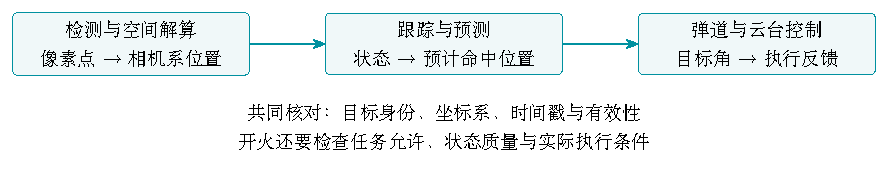
\includegraphics[width=0.95\textwidth]{aim_chain_revised.pdf}
\caption{自瞄三段链路；每段输出都要带上能供下一段解释的约定}
\label{fig:v3-aim-chain}
\end{figure}

先别急着问哪种算法最强，我们要先问怎样判断系统有用。偶尔打中一发当然很开心，不过它只能说明这一发打中了。比较两套方案时，还要记录命中次数与样本量、失跟情况、端到端延迟、距离、目标运动和光照，以及实际使用的配置版本；要比较算法本身，就尽量保持场景与条件一致。否则换了相机、目标和灯光以后效果好了，你很难知道是谁立的功。

\begin{example}[把结果指标拆开]
先填写两份教学记录：A为20次中12次、失跟0次、延迟10--20 ms、亮光；B也是20次中12次，但失跟6次、延迟10--60 ms、暗光。两份都只有60\%命中率，却暴露了不同的问题。接下来指出这份比较还缺什么：光照不一致，不能据此认定A的算法一定优于B。你已经把“能描述结果”和“能归因于改动”分开了。
\end{example}

\begin{exercise}
\label{v3-ex-aim-1}
命中率相同的两次实验，还应记录哪三类信息才能比较稳定性？如果测试光照不同，还能直接把差异归因于算法吗？
\end{exercise}

\subsubsection{目标检测（概述）}

首先我们要从图像里得到可以解算的观测。网络可能给出框和类别，传统处理可能给出灯条轮廓，最终用于几何解算的通常是有明确对应关系的图像点。两条路线怎样配合见上一章；这里不要把“找到了一个框”误认为“已经知道它在三维空间里哪里”。

接下来常用透视 n 点位姿估计（Perspective-n-Point，PnP）：准备目标的三维模型点、对应的二维像点、相机内参和畸变参数，求出模型系到相机系的旋转和平移。注意这个方向，相机安装在云台上并不会让两个坐标系自动变成同一个；要转到云台系，还需要安装外参和相关时刻的变换。\href{https://docs.opencv.org/4.x/d5/d1f/calib3d_solvePnP.html}{OpenCV 的 PnP 文档}解释了这一输出约定，具体计算回卷二几何视觉章。

\begin{example}[检查 PnP 输入清单]
在纸上画一个宽0.20 m、高0.10 m的教学矩形，它不代表赛场装甲尺寸。按左上、右上、右下、左下顺序写四个模型点：$(-0.10,-0.05,0)$、$(0.10,-0.05,0)$、$(0.10,0.05,0)$、$(-0.10,0.05,0)$。设相机系x向右、y向下、z向前，焦距均为600 px，主点$(320,240)$，畸变为0。模型与相机朝向一致，原点位于相机前方2 m时，四个像点应依次为$(290,225)$、$(350,225)$、$(350,255)$、$(290,255)$。先逐点连线，再故意交换第2、3个像点，你会看到物理对应已经变了。检查输入点序要在滤波之前，不能指望后面的平滑把错的对应关系修好。
\end{example}

\begin{note}
图像缩放或裁剪后，内参的像素尺度与主点可能需要一起变；目标模型用米，平移才按米解释。PnP能返回一个数值解也不等于输入正确，还要看重投影、正深度、点序和目标身份，卷二已经给出了可运行的正例与反例。
\end{note}

\begin{exercise}
\label{v3-ex-aim-2}
相机型号没变，但图像缩放到原来的一半，能直接沿用原像素尺度的内参吗？在上面的教学数据中写出新的焦距、主点和一个像点；若还裁剪了图像，应继续核对什么？
\end{exercise}

\subsubsection{目标跟踪与预测（概述）}

有了单帧位置以后，你很快会遇到位置跳变、遮挡和丢帧。跟踪器利用历史观测与运动模型继续估计状态，预测器再把状态推到需要的时刻。整车旋转时，可见装甲还会切换，不能总把某一块板当成永远沿直线走的小方块。整车模型是常见思路，但模型怎样选、什么时候失效，仍要靠对应数据验证。

丢一帧还可以沿模型预测，不过观测长期缺失时，不确定性会增长，目标也可能改变运动。你需要给状态标出质量和失效条件，不能因为还能输出坐标就一直允许开火。

卡尔曼滤波（Kalman Filter）和扩展卡尔曼滤波（Extended Kalman Filter，EKF）等负责带噪声的状态估计，细节见卷二滤波章。不过先学会滤波器的名字还不够，\textbf{状态属于哪个时刻}要一起记。状态已经外推过，时间戳却还是旧值，后面可能再补偿一次，同样的延迟就被算了两遍。

\begin{figure}[H]
\centering
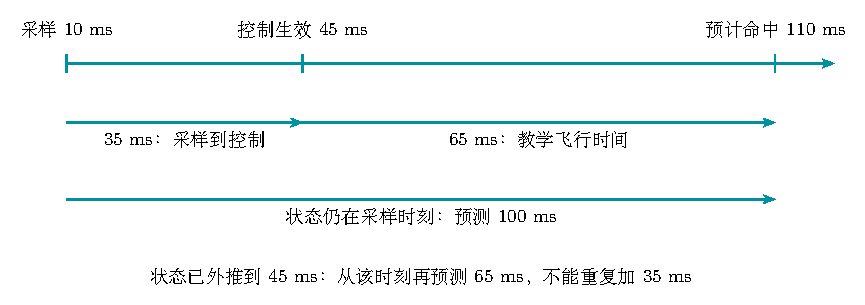
\includegraphics[width=0.95\textwidth]{aim_time_revised.pdf}
\caption{教学预测时间线：先确定状态时刻，再算到预计命中时刻的时长}
\label{fig:v3-aim-time}
\end{figure}

本卷的 \path{examples/aim-replay-demo/} 用 \texttt{replay.py} 演示时间线与中间量取证，\texttt{frames.csv} 提供五帧人工构造的回放。它只用 Python 标准库，不实现完整检测、滤波或控制。先看程序前半段，位置取4 m、速度取2 m/s，只做匀速外推，让你把时间语义看清楚：

\lstinputlisting[language=Python,basicstyle=\ttfamily\small,frame=single,breaklines=true,numbers=none,aboveskip=8pt,firstline=1,lastline=24]{examples/aim-replay-demo/replay.py}


\texttt{state\_at} 选采样时刻或控制生效时刻。选后者时，程序先更新位置，再更新状态时刻，然后用命中时刻减去状态时刻。\texttt{wrong\_repeat\_delay\_x\_m} 则故意计算“状态已前推却又把总延迟加一次”的反例，不能把它当成实际指令。

\begin{example}[画一条预测时间线]
在卷三目录进入项目，Python 3.10及以上即可运行：
\begin{tbash}
cd examples/aim-replay-demo
python3 replay.py
python3 replay.py --state-at control
\end{tbash}
默认采样10 ms，35 ms后控制生效，再飞行65 ms，所以预计命中为110 ms。若状态仍在10 ms，就预测100 ms，得到4.2 m；第二条命令把状态先推到45 ms，位置成为4.07 m，只再预测65 ms，同样得到4.2 m。反例却得到4.27 m，多出来的0.07 m正是重复补偿的35 ms乘速度。终端后面的回放检查稍后再读，先把这三个时刻画在同一条时间线上。
\end{example}

\begin{conclusion}
状态估计与未来预测是相连的两步。先问状态现在属于哪个时刻，再问预计命中在哪个时刻，二者的差才是还要外推的时间。飞行时间取定值和匀速运动只是本实验假设；实车上的旋转装甲、时变延迟与弹道求解，不能靠这个直线例子宣布已解决。
\end{conclusion}

\begin{exercise}
\label{v3-ex-aim-3}
采样到控制生效为25 ms，飞行60 ms。状态定义在采样时刻时，向前预测多久？若已外推到控制生效时刻呢？运行25/60 ms变式，核对两种状态时刻的预测位置。
\end{exercise}

\subsubsection{云台控制（概述）}

这时候我们有了期望方向，云台却不一定能马上转过去。弹道补偿处理飞行时间、下坠等问题，执行器控制处理从指令到实际转角的动态过程；惯量、角速度或加速度限制、延迟和机械间隙都可能影响到位。看到画面里目标跳了一下，就要求云台瞬间跳到新角度，云台也得有这个本事才行。

模型预测控制（Model Predictive Control，MPC）可以在模型与约束下选择一段控制序列，滚动执行；卷二已经讲了它怎样折中误差和控制量。这里先记住，算法优化不能消除执行器的物理限制，也不能替代实际反馈、限位与失效策略。

\begin{example}[检查限幅造成的滞后]
先在纸上写目标20度、当前0度、教学最大角速度100度每秒。忽略加减速，转完20度至少要0.2 s；10 ms内按这个上限只能转1度。检测再准确，也不能让它在10 ms内完成20度动作。这个结果是理想下界，实际延迟与加减速可能让到位更慢，并不是给真实云台设定参数。
\end{example}

\begin{exercise}
\label{v3-ex-aim-4}
同样条件下目标角改为15度，最短转动时间是多少？为什么这只是理想下界？若日志只有目标角，没有实际角反馈，能据此证明已经到位吗？
\end{exercise}

\subsubsection{最小二乘统一视角（导读）}

学到这里，你可能发现几何、滤波和控制都在说“让误差小一些”。这个共同视角能帮我们读算法，不过别顺手把束调整（Bundle Adjustment，BA）、Kalman和MPC当成同一个问题。BA调整几何量，让投影更贴近图像观测；Kalman在模型与噪声假设下递推估计状态；MPC在模型、代价和约束下选择未来控制。变量、依据和输出都不同，代价也不必总是简单的平方和。

\begin{example}[按误差对象认算法]
在纸上写三个现象：“投影与像点不一致”“带噪观测与状态预测不一致”“未来轨迹偏离参考且控制过大”，分别连到BA、Kalman、MPC，再补上它调整的是几何量、状态估计还是控制序列。连完后检查：把滤波器换成BA，并不能自动得到下一周期该发的控制指令。需要实现时，回卷二几何视觉、滤波与MPC章找对应项目。
\end{example}

\begin{exercise}
\label{v3-ex-aim-5}
把重投影误差、状态不确定性、轨迹与控制代价分别对应到BA、Kalman、MPC，并各写一种输出；为什么它们不能仅因都有误差就互换？
\end{exercise}

\subsubsection{沿链路保留证据}

最后我们回到调车时最常听见的话：“云台抖了。”这个现象太靠后了，前面的观测、解算、状态和指令都可能影响它。首先把同一目标、同一时刻附近的中间量放到一起，找哪一段最早出现变化，然后再回看原图或对应日志。时间先后能告诉你去哪里取证，不能只凭一列先跳就断言根因已经找到。

项目里的五帧回放如下，各列是为了讲明白传播顺序而人工填写的，\textbf{不是真实实车日志，也不是程序运行检测器或滤波器得到的输出}：
\lstinputlisting[basicstyle=\ttfamily\small,frame=single,breaklines=true,numbers=none]{examples/aim-replay-demo/frames.csv}

\texttt{first\_changes} 比较相邻行，分别用50 px、0.5 m、0.5 m、10度作教学变化阈值，保存每列第一次超过阈值的帧号。它没有判断误检或遮挡的能力，只是把值得回看的位置列出来。下面是剩余完整代码；命令行部分把时间线和回放结果一起输出：
\lstinputlisting[language=Python,basicstyle=\ttfamily\small,frame=single,breaklines=true,numbers=none,firstline=25]{examples/aim-replay-demo/replay.py}

\begin{example}[追到最早可见的变化]
仍在项目目录运行 \texttt{python3 replay.py}，四列的首个超阈值帧依次为120、120、121、122。先回看120帧的原图、角点及空间解算，而不是先换控制器。接下来运行 \texttt{python3 replay.py --pixel-threshold 150}，角点列变成 \texttt{null}；因为129 px没超过新阈值，不是因为角点已经恢复正常。真实异步链路要按时间戳对齐，不能直接拿行号替代时间。
\end{example}

\begin{conclusion}
观测可能有误检和模糊，解算可能有标定与对应错误，状态估计可能有模型失配，控制则受延迟与执行器约束。保留中间量以后，我们能缩小下一步调查范围；改阈值让告警消失，不等于把问题修好了。
\end{conclusion}

\begin{exercise}
\label{v3-ex-aim-6}
实际运行默认与150 px阈值变式，保存四列首个变化帧。指出下一步要保留的两类原始证据，并分别写一句“当前能判断什么”和“当前还不能判断什么”。
\end{exercise}


\section{本章小结}
\begin{conclusion}
从图像观测走到空间量，再走到状态、预测和控制，每一步都要检查身份、坐标与时间。你要能把采样、控制生效和预计命中画在同一条时间线上，用回放指出最早可观察的变化，再决定去哪里取证。具体PnP、滤波和MPC实现回卷二查；教学匀速例子与人工日志帮你核对链路，实车命中与云台响应仍要另做测量。
\end{conclusion}

\begin{problemset}
\item \label{v3-prob-aim-1}\textbf{基础题}：一次测试只报告“打中了”，缺少哪些信息才能说明系统有效？
\item \label{v3-prob-aim-2}\textbf{基础题}：PnP 需要哪些输入？其输出能直接当作云台系目标位置吗？
\item \label{v3-prob-aim-3}\textbf{基础题}：丢失一帧后，跟踪器为什么仍可给出状态？为什么又不能无限相信它？
\item \label{v3-prob-aim-4}\textbf{基础题}：为什么弹道补偿正确，云台仍可能无法及时跟上目标？
\item \label{v3-prob-aim-5}\textbf{基础题}：“BA、Kalman、MPC 都是在解同一个最小二乘问题”是否准确？
\item \label{v3-prob-aim-6}\textbf{提高题}：角点在第 120 帧跳变，空间位置随后跳变，云台最后抖动。先检查哪一段，保留什么证据？
\item \label{v3-prob-aim-7}\textbf{实践题}：在本机新建一份时间线记录：采样 10 ms、控制生效 45 ms、飞行 65 ms。算出目标命中时刻与从采样时刻起的预测时长，并注明假设。
\end{problemset}

\section{本章验收}
\begin{enumerate}
  \item 用一页图向学长讲清检测、跟踪预测、云台控制三段，并在每段标出一个主要噪声来源。
  \item 在给定回放上选择一个异常时刻，展示至少两段中间量，说明证据能支持和不能支持的故障判断。
\end{enumerate}

\chapter{导航在 RM 中的应用}
\begin{introduction}
  \item 学习目标：说明地图、定位、规划、控制与恢复的分工，按证据定位常见故障。
  \item 建议学时：约 2--3 小时，含纸面地图与实际Nav2日志核对。
  \item 本卷边界：只讲比赛任务与接口；建图、坐标变换和 Nav2 配置见卷二导航章。
\end{introduction}
\label{ch:v3-nav}

\section{比赛任务与导航模块}
\section{比赛故事：从「缺德地图」到 Nav2}

想象你坐在哨兵「脑袋」里要去偷家：需要一张赛场地图、知道自己在哪、算出一条路，边走边躲动态障碍。
这正是导航方向在 RM 中的缩影。算法细节见卷二「导航与 SLAM」；本章只讲\textbf{比赛语义}。

\section{赛场上的模块含义}

对照 Nav2 一类框架，比赛中常见对应关系：

\begin{enumerate}
    \item \textbf{地图}：赛前建图环节得到的静态层 + 比赛中代价地图动态层；
    \item \textbf{定位}：激光雷达 / 里程计 / IMU 等融合（此处「雷达」指 \textbf{LiDAR 传感器}，不是雷达站方向）；
    \item \textbf{全局规划}：在已知地图上找大致路线；
    \item \textbf{局部规划 / 控制}：躲突然出现的障碍，输出速度指令给电控；
    \item \textbf{恢复行为}：卡住后旋转、后退、清代价地图、重规划等；
    \item \textbf{行为树}：编排「规划—跟随—恢复」的比赛逻辑，而不是写死巨型 if-else。
\end{enumerate}

\begin{figure}[H]
    \centering
    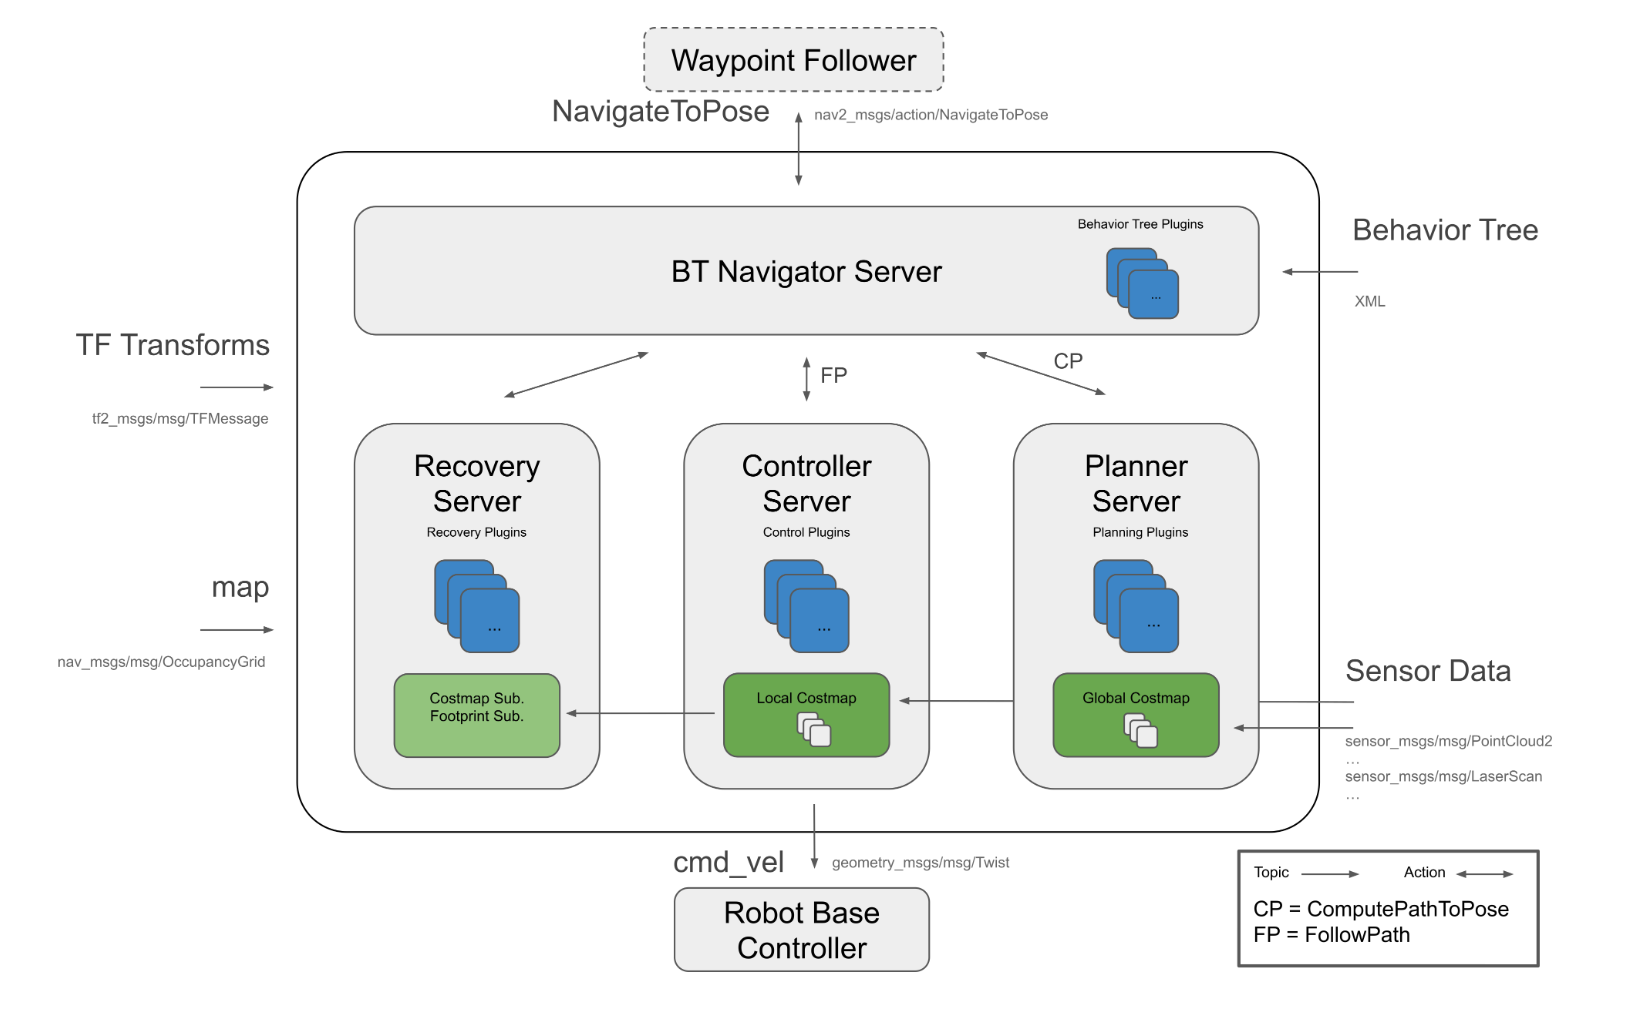
\includegraphics[width=0.85\textwidth]{Nav2导航框架.png}
    \caption{Nav2 导航框架示意（细节回卷二）}
    \label{fig:v3_nav2}
\end{figure}

\section{建图与比赛流程}

\begin{itemize}
    \item 赛前按规则完成哨兵建图，检查噪声黑点、禁行区是否涂正确；
    \item 赛中代价地图必须反映新障碍；膨胀层要按车体尺寸设置，避免「规划成功但车体擦墙」；
    \item 动态障碍（其它机器人等）主要靠局部层与恢复行为，不能只信全局静态图。
\end{itemize}

\section{与雷达、决策的接口}

导航消费「我在哪、路怎么走」；雷达站提供的全场目标位置可辅助战术决策，但\textbf{坐标系统、单位、延时}必须与队内约定一致。
导航不负责高台俯视检测；雷达不负责底盘速度闭环。

\section{故障对照（验收提示）}

| 现象 | 优先怀疑 |
|------|----------|
| 全局路线穿墙 | 地图/膨胀/全局规划器 |
| 有路但贴障发抖 | 局部规划或控制频率 |
| 卡住原地转圈 | 恢复行为配置或代价地图未清 |
| 位姿跳变丢定位 | TF / 定位源融合 |
| 指令有但不走 | 与电控接口或急停 |

验收：对照框图，能把上述现象归到 [1]--[6] 中的一类模块。


\section{本章小结}
\begin{conclusion}
从“想去哪”走到“现在怎样动”，中间还有自身定位、环境表达、路径与实际执行。你需要能在地图上认出这些职责，核对尺寸与坐标，再用真实保存的结果分清失败发生在哪一层。卷二提供实际Nav2软件工程，实车的定位、动态观测、制动和恢复前提仍要另外测量；本章的纸面棋子和软件模型不能代替它们。
\end{conclusion}

\begin{problemset}
\item \label{v3-prob-nav-1}\textbf{基础题}：去补给点的任务中，目标点、全局路径、速度指令分别回答什么问题？
\item \label{v3-prob-nav-2}\textbf{基础题}：地图、定位、行为树能相互替代吗？分别举一个输入或输出。
\item \label{v3-prob-nav-3}\textbf{基础题}：为什么静态地图正确仍需更新局部障碍？
\item \label{v3-prob-nav-4}\textbf{基础题}：导航能否把雷达广播中的敌方坐标直接当成自身定位？
\item \label{v3-prob-nav-5}\textbf{提高题}：全局路径穿墙与“指令有但不走”分别优先检查哪些证据？
\item \label{v3-prob-nav-6}\textbf{实践题}：在本地保存一张纸面地图照片或绘图文件，标出车体尺寸、通道宽度和一处动态障碍；对一个直通道作宽度核算。
\end{problemset}

\section{本章验收}
\begin{enumerate}
  \item 对照 Nav2 框图讲清全局规划、局部控制与恢复的分工；学长临时改变障碍位置后重新解释流程。
  \item 给定一段卡住的日志或回放，当场指出两个候选模块并展示下一步取证位置，不凭现象直接定责。
\end{enumerate}

\chapter{雷达站与全场感知概述}
\begin{introduction}
  \item 学习目标：画出雷达站数据流，区分平面映射和 PnP，按明确条件选择有效坐标。
  \item 建议学时：约 2--3 小时，含平面映射与选源实跑。
  \item 本卷边界：可选无线电与反制链路仅作架构示例，是否采用须核对参赛赛季规则；实现见卷二通信、SDR 与视觉相关章。
\end{introduction}
\label{ch:v3-radar}

\section{全场定位、通信与时效}
\subsubsection{雷达站是什么}

\textbf{雷达}方向：利用场地高处视角与算力，识别全场目标等信息，经裁判系统向队友共享。
它与导航章中的\textbf{激光雷达（LiDAR）}不是同一概念。

与自瞄的核心差异：
\begin{itemize}
    \item 自瞄：单车、近距、云台闭环、持续跟瞄；
    \item 雷达：全场、多目标、俯视几何、\textbf{广播}为主，不直接拧本车云台。
\end{itemize}

\begin{example}[区分站与传感器]
写下“高台相机识别目标并共享坐标”和“车载 LiDAR 量测墙面帮助定位”，圈出最终输出：前者是全场目标信息，后者服务本车位姿。检查：名称含“雷达”并不能说明承担同一种比赛任务。
\end{example}

\begin{exercise}
\label{v3-ex-radar-1}
一套高台视觉系统没有 LiDAR，还可以属于雷达方向吗？说明依据。
\end{exercise}

\subsubsection{典型软件架构（概述）}

可把软件拆成以下教学架构；其中无线电与反制均为可选示意，不代表每个赛季都有相同任务或权限：
\begin{enumerate}
    \item \textbf{地面视觉}：工业相机 → 检测/跟踪 → 场地图坐标 → 融合 → 裁判串口；
    \item \textbf{无线电（可选）}：软件定义无线电（Software Defined Radio，SDR）按适用协议接收与解析信息，经本机 TCP 交给视觉；
    \item \textbf{反制（可选）}：长焦检测与云台，和地面端用独立串口同步次数。
\end{enumerate}

通信模式见卷二「多机通信」；SDR 与解析见卷二「SDR 与电磁波解析」。本卷只要求能画数据流并说出职责边界。

数据流可记为：工业相机经识别跟踪得到场地图坐标；可选的 SDR 解码坐标按新鲜度与视觉融合后，经裁判系统广播；反制计数为可选旁路。

\begin{figure}[H]
\centering
\resizebox{0.9\textwidth}{!}{%
\begin{tikzpicture}[box/.style={draw=cyan!60!black,rounded corners,align=center,
  minimum height=11mm,text width=27mm,fill=cyan!5},>=stealth]
\node[box] (vision) at (0,1) {视觉检测与映射\\场地系坐标};
\node[box,dashed] (radio) at (0,-1) {可选无线电解析\\有效坐标};
\node[box] (fusion) at (4.2,0) {身份、质量与时效\\检查后选源};
\node[box] (send) at (8.4,0) {协议封装与广播\\坐标或无效状态};
\draw[->,thick] (vision.east) -- (fusion.west);
\draw[->,thick,dashed] (radio.east) -- (fusion.west);
\draw[->,thick] (fusion) -- (send);
\end{tikzpicture}}
\caption{雷达站坐标主路；需按序处理的事件不与最新坐标共用覆盖队列}
\label{fig:v3-radar-chain}
\end{figure}

\begin{example}[把旁路从主路分开]
画出视觉进程 → 融合 → 广播三框，再从可选无线电进程画箭头接到融合。用手遮住无线电框，检查主路是否仍能输入视觉坐标；再给非坐标事件单画一条有序处理支路。检查：可选模块故障不应在设计上阻塞仍有效的坐标主路。
\end{example}

\begin{exercise}
\label{v3-ex-radar-2}
为何坐标可以只保留最新值，反制计数或任务事件却不能随意覆盖？
\end{exercise}

\subsubsection{俯视定位 vs 车载 PnP}

雷达可用场地图关键点与单应变换（Homography）或区域映射，把适用平面上的图像点映射到场地坐标；有高度差时需分区域、补充高度信息或使用三维方法验证，不能把任意车顶像素都当作地面点。
自瞄常用装甲板模型 + PnP 求相对位姿。二者标定物、误差来源与调参方式都不同，不要混用术语。

检测上常见级联：车辆检测 → 装甲/灯条 → 数字分类；再接多目标跟踪。细节回卷二 B/C。

\begin{example}[验证平面假设]
在教学场地图上标出四个任意三点不共线的地面角点，声明它们是图像与场地的对应点。再选一个未参与标定的地面点检查映射误差。把验证点移到高台上后，标注“高度不在同一平面，原映射不保证有效”。检查：映射适用范围必须写在配置旁。
\end{example}

\begin{exercise}
\label{v3-ex-radar-3}
直接把车顶检测框中心用地面单应映射到场地，为什么可能产生偏差？
\end{exercise}

\subsubsection{融合与时效}

若存在无线电坐标，可采用一种教学策略：先检查身份、坐标系、质量与时效，再让\textbf{合格且新鲜的无线电优先}；否则回退有效视觉或显式标记无效。这不是所有系统通用的优先级。
非坐标事件可走独立处理通道，避免阻塞坐标。坐标可采用只保留最新值（latest-value）的方式；计数增量、事件或需确认的消息不能直接套用覆盖策略。

对队友有用的是「对的坐标系 + 可接受延迟」；错系、堵包、过期坐标比「偶尔缺一帧」更具破坏性。

\begin{example}[按有效性与时效选源]
教学策略：同一目标、同一坐标系且质量合格时，无线电年龄不超过 100 ms 则优先；否则选择年龄不超过 150 ms 的视觉；二者均不合格就输出无效。当前时刻 1000 ms，无线电采样于 850 ms，视觉采样于 950 ms，年龄分别为 150、50 ms，应选视觉。这些阈值仅用于演练。
\end{example}

\begin{note}
本章不提供当年比赛的功能授权、频率或协议常量。无线电、反制与裁判广播须由负责人核对参赛赛季官方规则与协议后采用。平面映射前提见 OpenCV 官方说明：\url{https://docs.opencv.org/4.x/d9/dab/tutorial_homography.html}。
\end{note}

\begin{conclusion}
\begin{itemize}
  \item 先确认同一目标与坐标，再检查质量与年龄，最后选源。
  \item 接收时刻不等于采样时刻。
  \item 两源均无效时明确报告失效。
\end{itemize}
\end{conclusion}

\begin{exercise}
\label{v3-ex-radar-4}
沿用示例策略，当前 1000 ms，无线电采样 930 ms 但校验失败，视觉采样 960 ms 且有效，选谁？若视觉也过期呢？
\end{exercise}

\subsubsection{技能映射}

\begin{center}
\begin{tabular}{@{}p{0.30\textwidth}p{0.62\textwidth}@{}}
\toprule[1.5pt]
能力 & 卷二 \\
\midrule[1pt]
节点与工程 & ROS2 \\
TCP/串口/裁判帧 & 多机通信 \\
SDR/IQ/状态机 & SDR 与电磁波解析 \\
检测与跟踪 & OpenCV、深度学习 \\
相机与标定 & 相机成像 \\
部署加速 & CUDA \\
\bottomrule[1.5pt]
\end{tabular}
\end{center}

\begin{example}[沿故障查专项]
教学问题是“识别框稳定，队友收到的位置总是很旧”。先沿发送队列、融合取值、接收消费画检查点，再到卷二多机通信查最新值与故障隔离。检查：此时优先补通信知识，比立即换检测模型更直接。
\end{example}

\begin{exercise}
\label{v3-ex-radar-5}
若画面上目标清楚但数字类别经常错，应先查卷二哪些章？若坐标正确但串口帧被拒收呢？
\end{exercise}


% 章末复习与验收集中排版，避免末页只剩一个条目。
\clearpage
\section{本章小结}
\begin{conclusion}
我们先用全场观测回答目标是谁，再在明确的几何前提下换算坐标，最后把合格而新鲜的信息共享出去。你需要能说清雷达站与LiDAR的任务差别，运行高度偏差和选源例子，解释为什么同样两个数字有时可用、有时必须拒绝。现场标定、可选功能和广播限制仍要用真实设备及适用规则验证；具体工程回卷二与队内版本化文档。
\end{conclusion}

\begin{problemset}
\item \label{v3-prob-radar-1}\textbf{基础题}：雷达站与自瞄的主要输出及闭环对象有什么不同？
\item \label{v3-prob-radar-2}\textbf{基础题}：多进程链路中，无线电进程退出后，视觉仍正常，融合进程应如何处理？
\item \label{v3-prob-radar-3}\textbf{基础题}：地面单应映射与装甲 PnP 的输入约束各是什么？
\item \label{v3-prob-radar-4}\textbf{基础题}：来自两台未同步机器的时间戳能直接相减判断观测年龄吗？
\item \label{v3-prob-radar-5}\textbf{基础题}：检测正常而广播持续积压，应优先回卷二查哪类内容？
\item \label{v3-prob-radar-6}\textbf{提高题}：有效无线电年龄 120 ms，视觉年龄 160 ms。按本章 100/150 ms 阈值应输出什么？若无线电年龄恰为 100 ms 呢？
\item \label{v3-prob-radar-7}\textbf{实践题}：在本机保存一张选源表，覆盖有效无线电、无线电过期、无线电无效、两源均无效四种情况，记录输入年龄与输出。
\end{problemset}

\section{本章验收}
\begin{enumerate}
  \item 口述雷达站输入输出，画出视觉与可选无线电的数据流，并分别说清与自瞄、导航的职责边界。
  \item 学长现场给出两源的有效性与时间状态，演示如何判定过期与回退，同时解释 LiDAR 与雷达方向的区别。
\end{enumerate}

\chapter{相机与前端的赛场实践要点}
\begin{introduction}
  \item 学习目标：执行相机检查清单，区分快门畸变与拖影，记录有效帧率和端到端延迟。
  \item 建议学时：约 2 小时，含相机或现成图像检查。
  \item 本卷边界：本章只讲现场检查；成像原理、标定与 SDK 编程见卷二相机章。
\end{introduction}
\label{ch:v3-camera}

\section{成像质量与采集检查}
\subsubsection{原则：原理在卷二，本章是 检查清单}

曝光三角、卷帘快门、噪声等原理见卷二「相机与成像」。本章只列赛场上最常踩坑的实践要点。

\begin{example}[建立一次检查记录]
准备一张表，写入日期、相机序列号、镜头、分辨率、曝光、增益、触发方式与标定文件。没有设备时填写“未核对”并注明需查的配置来源。检查：这张表应让另一位同学知道哪些条件已确认，而不是只留下“相机正常”。
\end{example}

\begin{exercise}
\label{v3-ex-camera-1}
检查表中只写“海康相机，默认参数”，为什么不能复现实验？列出四项缺失信息。
\end{exercise}

\subsubsection{卷帘 vs 全局}

\begin{itemize}
    \item \textbf{卷帘快门（Rolling Shutter）}：高速相对运动时易倾斜、撕裂，影响角点与检测稳定性；
    \item \textbf{全局快门（Global Shutter）}：运动场景更稳，成本与选型受限。
\end{itemize}
自瞄对抗、云台快速扫场时，快门类型与曝光时间必须一起评估：曝光过长同样拖影。

\begin{example}[分开观察畸变与拖影]
在已有的快速扫场图像中，分别检查竖直边缘是否整体倾斜、单个灯条边缘是否沿运动方向拉长。前者提示逐行曝光时序效应，后者提示曝光期间运动模糊。记录现象，再用固定其他条件、缩短曝光的对照图检查拖影是否减轻。没有对照图时，只记录候选原因。
\end{example}

\begin{exercise}
\label{v3-ex-camera-2}
全局快门图像仍有明显拖影，能否据此判定相机实际是卷帘快门？
\end{exercise}

\subsubsection{分辨率、帧率与「商家高清」}

\begin{itemize}
    \item 宣传「高清」不等于赛场可用分辨率；
    \item 帧率常与分辨率绑定：高帧可能对应较低分辨率；
    \item 端到端延迟应覆盖约定采样时刻到执行生效之间的读出、传输、排队、处理和执行等待；各阶段可能重叠，应以逐帧时间戳实测，不能用帧率的倒数代替。提高分辨率可能增加处理负担。
\end{itemize}
选型时写清：目标分辨率、最低可接受帧率、接口（USB3/GigE）、黑白/彩色、触发方式。

\begin{example}[用时间戳区分两个指标]
教学样本的连续采样时刻为 0、10、20 ms，对应结果输出时刻为 35、45、55 ms。采样间隔 10 ms，对应 100 帧每秒；逐帧延迟为 35 ms。检查：流水线可每 10 ms 出一帧结果，但每个结果仍反映 35 ms 前的观测。
\end{example}

\begin{exercise}
\label{v3-ex-camera-3}
采样时刻为 0、20、40 ms，结果输出为 50、70、90 ms，采样帧率和逐帧延迟分别是多少？
\end{exercise}

\subsubsection{曝光 / 增益 / 触发 检查清单}

上机前逐项确认：
\begin{enumerate}
    \item 灯条不过曝成一片、暗部仍可见结构；
    \item 增益过高引入的噪声是否拖垮阈值/网络；
    \item 是否已验证曝光策略；自动曝光若拉长曝光或改变灰度分布，可能影响高速运动检测，可锁定曝光或限制自动范围并作对照；
    \item 硬件触发 / 同步是否与电控时间戳约定一致；
    \item 镜头焦距与工作距离是否匹配装甲成像尺寸；
    \item 内参与畸变是否在本机标定，配置是否写对序列号。
\end{enumerate}

雷达俯视与车载自瞄的工作距离、视场（FOV）不同，\textbf{禁止}共用一套未经验证的曝光参数。

\begin{example}[一次只改曝光]
用同一段场景准备两组图像，固定镜头、增益和分辨率，仅改变曝光；记录灯条是否饱和、边缘拖影和暗部可见性。选择兼顾检测与运动条件的一组，保存配置和样图。检查：没有统一的“越亮越好”；缺少设备时可对已有对照图作同样记录。
\end{example}

\begin{note}
切换曝光、触发或采集模式前先保存配置；上机检查时保持执行器处于约定的安全状态。快门类型原理可查厂家说明：\url{https://docs.baslerweb.com/electronic-shutter-types}；实际参数名称与范围以本机型号手册为准。
\end{note}

\begin{conclusion}
\begin{itemize}
  \item 快门类型决定各行曝光的时序关系。
  \item 曝光时长影响拖影和亮度。
  \item 帧率表示采样吞吐，端到端延迟表示某次观测到执行的耗时。
\end{itemize}
\end{conclusion}

\begin{exercise}
\label{v3-ex-camera-4}
换了焦距或裁剪区域后，除了曝光还应核对哪项几何配置？为什么？
\end{exercise}

\subsubsection{工业相机与 SDK*}

赛场常用厂家软件开发工具包（Software Development Kit，SDK，如海康相机 SDK）按序列号打开，而不是笼统 \texttt{VideoCapture(0)}。
驱动、权限、USB 带宽不足时会丢帧——先查系统层再查算法。

\begin{example}[确认打开的是哪台相机]
在厂家查看器中只启动采集预览，读取序列号并与配置文件对照；保存一帧图像，记录分辨率与时间信息，再退出查看器释放设备供程序使用。检查：预览可用仅证明这一采集路径可用，正式程序仍需验证权限、像素格式和时间戳。
\end{example}

\begin{exercise}
\label{v3-ex-camera-5}
查看器能出图而算法程序打不开设备，先检查什么？
\end{exercise}


% 章末复习与验收集中排版，避免末页只剩一个条目。
\clearpage
\section{本章小结}
按相机身份与配置、成像质量、帧流时效、后端输入的顺序检查前端。必须会区分快门类型与曝光时长、采集帧率与端到端延迟；型号参数与 SDK 细节按对应设备手册查阅。

\begin{problemset}
\item \label{v3-prob-camera-1}\textbf{基础题}：一份前端检查记录至少应覆盖哪三类信息？
\item \label{v3-prob-camera-2}\textbf{基础题}：卷帘几何畸变与长曝光拖影分别由什么机制引起？
\item \label{v3-prob-camera-3}\textbf{基础题}：相机能采集 120 帧每秒，为什么不能据此宣称系统延迟只有约 8.3 ms？
\item \label{v3-prob-camera-4}\textbf{基础题}：自动曝光使静止画面更亮，为什么不能直接证明它适合高速对抗？
\item \label{v3-prob-camera-5}\textbf{基础题}：相机序列号与标定文件不匹配时，即使检测框正常，还可能出什么问题？
\item \label{v3-prob-camera-6}\textbf{提高题}：同时增大分辨率、曝光和增益后漏检减少，但云台更滞后，该如何拆分验证？
\item \label{v3-prob-camera-7}\textbf{实践题}：用一张本地图片或一段录包做前端检查，保存原始文件路径、图像尺寸、饱和与拖影的观察及缺失的采集元数据。
\end{problemset}

\section{本章验收}
\begin{enumerate}
  \item 现场按清单检查一台相机，演示一项曝光或触发设置的读取与确认，并说明改动如何保存和恢复。
  \item 面对学长提供的型号页和实际帧流记录，说明标称高帧率为何不保证实用，指出当前证据仍缺哪项。
\end{enumerate}

\chapter{工程准则与调车文化}
\begin{introduction}
  \item 学习目标：复述五条准则，编写可复现测试记录，并据证据安排一次单变量验证。
  \item 建议学时：约 1.5 小时；开营与结营各复习一次。
  \item 本卷边界：本章规定开发和协作过程；具体调参与测试脚本回卷二和方向仓库。
\end{introduction}
\label{ch:v3-engineering}

\section{五条准则与问题定位}
\subsubsection{为何本卷必读本章}

算法理论只是冰山一角。赛场成败往往取决于工程习惯与协作方式。
下列五条凝练自队内调车经验（源自自瞄核心算法讲义结语），开营与结营各读一次；培训负责人可据此做过程检查。

\begin{example}[把“好了”改写成证据]
原记录是“今天调好了”。改成“固定录包 A，配置版本 B，目标帧范围 100--150，修改前位置有三次跳变；本次只调整角点筛选，修改后同区间无跳变，尚未实车验证”。检查：他人可以找到输入、修改和比较对象，且不会误把回放成功当作已通过实车。
\end{example}

\begin{exercise}
\label{v3-ex-engineering-1}
一项改动只在仿真中通过，记录中应怎样写结论与下一步？
\end{exercise}

\subsubsection{五条准则}

\begin{enumerate}
    \item \textbf{实测优先，仿真为辅。}
    仿真难以复现真实光照、振动、弹道散布与对手机动。新算法须经靶场与对抗演练再定稿。

    \item \textbf{边测边写，过程正确比结果正确更重要。}
    不要只盯最终命中率——偶然命中可能是「蒙对」。应逐环节检查：检测是否稳定、解算是否跳变、滤波是否收敛、控制是否平滑。每一步可复现，整体才可复现。

    \item \textbf{拒绝重复造轮子；重构是学习，调车是工作。}
    成熟的 PnP、Kalman、MPC、检测框架优先复用。为理解原理而重构关键模块属于\textbf{学习时间}；临场调车属于\textbf{工程时间}：稳定优先，用验证过的组件。

    \item \textbf{强化四项意识：时间、进度、合作、钻研。}
    视觉跨识别、估计、控制、机械接口，单人难通吃。设里程碑、定期同步消息与坐标系；难点查资料或请教，避免无效死磕。

    \item \textbf{先定位问题，再寻找解，切忌盲目乱试。}
    偏弹、抖动、跳变时，先用日志、可视化与离线回放锁定异常环节与时刻，再改参数或算法。随机拧参「蒙好」会在下一场暴露更多隐患。
\end{enumerate}

\begin{example}[按五条准则安排一次修改]
教学故障是扫场时位置跳变。先在现成录包上复现，逐段查看原图与角点；保留已验证的解算器，仅修改角点筛选；分配采集、分析与复核负责人；写下假设后做同一录包的对照。检查：五条准则分别落在证据、过程、复用、协作和定位上。
\end{example}

\begin{exercise}
\label{v3-ex-engineering-2}
临场前一天想重写已验证的滤波器，理由是“自己写更懂”。应如何安排学习与工程工作？
\end{exercise}

\subsubsection{过程检查表示意}

\begin{center}
\begin{tabular}{@{}p{0.72\textwidth}p{0.20\textwidth}@{}}
\toprule[1.5pt]
检查项 & 是 / 否 \\
\midrule[1pt]
本周改动是否有实车或录包证据 &  \\
是否能指出问题发生在检测/解算/滤波/控制哪一段 &  \\
接口变更是否更新了文档与消息定义 &  \\
是否区分了学习实验分支与比赛主分支 &  \\
\bottomrule[1.5pt]
\end{tabular}
\end{center}

\begin{example}[填写一条失败记录]
按检查表填入：输入录包 A、基线版本 B、单一改动 C、比较窗口和指标、结果恶化、恢复 B。即使改动失败，记录仍能排除一个假设。检查：失败结果保留，接口变更同时记录发送端和接收端验证。
\end{example}

\begin{note}
实车运动与开火测试须在队内规定场地和监督条件下进行，先确认急停、限位及人员位置。离线回放通过只能支持其覆盖的条件，不能直接记作实车已通过。
\end{note}

\begin{conclusion}
\begin{itemize}
  \item 固定基线，写下假设。
  \item 一次改变一个主要因素，比较同一输入下的中间量与结果。
  \item 保存失败实验与回滚记录。
\end{itemize}
\end{conclusion}

\begin{exercise}
\label{v3-ex-engineering-3}
测试结果变差后，删掉失败记录只留“最终好参数”有什么问题？
\end{exercise}

\subsubsection{适用范围}

五条不仅适用于自瞄，也适用于雷达站多进程联调与导航上图。从「能跑」到「能战」，靠的是可复现的过程，而不是单次好运。

\begin{example}[把准则迁移到导航]
把自瞄记录中的原图、角点和控制量替换为地图、位姿、路径和速度，仍按同样顺序记录版本、场景、最早异常与单一改动。检查：准则迁移的是取证方法，不能把自瞄阈值照搬到导航。
\end{example}

\begin{exercise}
\label{v3-ex-engineering-4}
雷达通信偶发积压时，“先定位再寻找解”应怎样落实？给出两个可观察量。
\end{exercise}


% 章末复习与验收集中排版，避免末页只剩一个条目。
\clearpage
\section{本章小结}
五条准则把算法开发变成可复现的协作过程：实测给证据，逐段观察解释结果，复用稳定组件控制变更，明确分工保障进度，先定位再验证避免盲改。必须熟练写记录与回滚条件，具体工具按卷一、卷二查阅。

\begin{problemset}
\item \label{v3-prob-engineering-1}\textbf{基础题}：仿真通过后仍需实测的两个原因是什么？
\item \label{v3-prob-engineering-2}\textbf{基础题}：为什么评价链路时不能只看最终命中率？
\item \label{v3-prob-engineering-3}\textbf{基础题}：学习时间的重构成果何时才适合进入比赛工程？
\item \label{v3-prob-engineering-4}\textbf{基础题}：“时间、进度、合作、钻研”各对应一项怎样的记录？
\item \label{v3-prob-engineering-5}\textbf{基础题}：一个合格的失败实验记录至少保留什么？
\item \label{v3-prob-engineering-6}\textbf{提高题}：换相机、换模型、改滤波参数后效果改善，能归因于哪一项？设计最小后续验证。
\item \label{v3-prob-engineering-7}\textbf{实践题}：在本地写一条导航或雷达问题的实验计划，包含假设、最早可观测异常、单一变量、通过条件与回滚条件。
\end{problemset}

\section{本章验收}
\begin{enumerate}
  \item 不看讲义复述五条准则标题，再用自己的经历解释为何只看最终命中率不够。
  \item 给学长演示一次从基线、复现、单变量验证到回滚的完整记录；由另一人按记录复核关键证据。
\end{enumerate}

\chapter{进阶地图与资料索引}
\begin{introduction}
  \item 学习目标：按方向列出学习路径，定位教材入口，并填写可追溯的资料与责任记录。
  \item 建议学时：约 1 小时，含本地索引检查。
  \item 本卷边界：本章只维护入口和版本；知识正文留在相应卷章，队内地址和人员由负责人确认。
\end{introduction}
\label{ch:v3-index}

\section{学习路径与资料维护}
\subsubsection{三卷分工}

\begin{center}
\begin{tabular}{@{}>{\raggedright\arraybackslash}p{0.21\textwidth}>{\raggedright\arraybackslash}p{0.43\textwidth}>{\raggedright\arraybackslash}p{0.24\textwidth}@{}}
\toprule[1.5pt]
卷 & 内容 & 何时读 \\
\midrule[1pt]
卷一 · 基础通识 & Linux、C++、CMake、Git & 入门必过 \\
卷二 · 专项技术栈 & ROS2、通信、SDR、OpenCV、深度学习、CUDA、相机、滤波、BA、MPC、导航 & 按方向选修 \\
卷三 · 本卷 & 赛场链路、接口边界、工程准则 & 开营精读 + 中期答辩 \\
\bottomrule[1.5pt]
\end{tabular}
\end{center}

\begin{example}[把问题放回正确卷册]
建立三行书签：卷一编译与 CMake、卷二几何视觉与 BA、卷三工程准则。分别给“链接错误”“PnP 点序”“联调前如何留证据”连线。检查：先按问题性质找入口，避免从头翻整套书。
\end{example}

\begin{exercise}
\label{v3-ex-index-1}
Git 操作不熟、坐标广播积压、调车没有版本记录，分别优先查哪卷？
\end{exercise}

\subsubsection{按方向的推荐顺序}

\textbf{自瞄（学习时间 $\rightarrow$ 工程时间）：}
卷一 $\rightarrow$ 本卷第\ref{ch:v3-overview}、\ref{ch:v3-aim}、\ref{ch:v3-engineering}章 $\rightarrow$ 卷二 ROS2、OpenCV、深度学习、相机、滤波、BA、MPC $\rightarrow$ 回本卷做链路答辩 $\rightarrow$ 实车仓库。

\textbf{雷达：}
卷一 $\rightarrow$ 本卷第\ref{ch:v3-overview}、\ref{ch:v3-radar}、\ref{ch:v3-engineering}章 $\rightarrow$ 卷二 ROS2、多机通信、SDR、OpenCV、深度学习、相机 $\rightarrow$ 开源/队内雷达仓库部署文档。

\textbf{导航：}
卷一 $\rightarrow$ 本卷第\ref{ch:v3-overview}、\ref{ch:v3-nav}、\ref{ch:v3-engineering}章 $\rightarrow$ 卷二 ROS2、导航（通信建议）$\rightarrow$ 建图与实车。

\begin{example}[给导航新人排顺序]
写出“卷一通识 → 本卷职责、导航、工程准则 → 卷二 ROS2 与导航 → 回到本卷答辩 → 受控实车”。在每一步旁标注输出：基础小工程、链路图、专项练习、现场演示。检查：学习计划包含产出，不能只有书单。
\end{example}

\begin{exercise}
\label{v3-ex-index-2}
雷达新人不会串口帧解析，是否应先因“看起来高级”而跳去 MPC？写出更直接的补课顺序。
\end{exercise}

\subsubsection{资料索引（活页）}

\begin{itemize}
    \item 卷二各章：\texttt{02-专项技术栈/}
    \item 自瞄公式与导读：\texttt{视觉培训/最小二乘法/}（讲义 + BA/Kalman/MPC）
    \item 雷达站参考实现：队内指定开源仓库与部署说明（注意许可证与权重策略）
    \item 相机 / 控制器 PPT、视觉小课堂：队内资料目录
    \item 裁判系统协议：当年官方文档（勿依赖过期拷贝）
\end{itemize}

\begin{example}[检查一个真实入口]
在本地文件浏览器依次打开项目目录、02-专项技术栈、main.tex，搜索“多机通信方法”，沿其 input 找到章节文件。记录入口、章名和检查日期。若队内讲义路径在本机不存在，记录“本机未取得访问入口”，交负责人确认。检查：书中提到的路径不等于当前电脑必定存在。
\end{example}

\begin{note}
队内仓库地址、接口责任人和复盘日期由负责人填写。本书不虚构这些信息；本机没有路径时应记录待确认，不要把未访问的资料标成已核验。
\end{note}

\begin{conclusion}
\begin{itemize}
  \item 路径回答在哪里，版本回答适用哪套实现。
  \item 责任人回答由谁确认，核对日期回答何时验证。
  \item 四项一起记录，才能让索引可追溯。
\end{itemize}
\end{conclusion}

\begin{exercise}
\label{v3-ex-index-3}
只有一个没有版本号的协议截图，够不够作为联调依据？还需取得什么信息？
\end{exercise}

\subsubsection{版本与责任}

\begin{center}
\begin{tabular}{@{}p{0.30\textwidth}p{0.62\textwidth}@{}}
\toprule[1.5pt]
项目 & 填写 \\
\midrule[1pt]
教材版本 & \texttt{2026.08} \\
本卷维护 & 视觉组培训负责人 \\
接口文档责任人 & （队内填写） \\
下次复盘日期 & （队内填写） \\
\bottomrule[1.5pt]
\end{tabular}
\end{center}
本章为活页：仅入口路径变化时更新本章即可；协议字段或行为变化时，还须同步接口文档、实现和验证，不能只换链接。

\begin{example}[完成一次索引变更]
教学情景：部署说明从路径 A 迁到 B。记录旧入口、新入口、适用分支或版本、检查日期与维护人；用新入口实际打开文档，再让另一位同学复核。无法访问 B 时记录受阻原因，不能标成已完成。
\end{example}

\begin{exercise}
\label{v3-ex-index-4}
教材活页改了协议链接，但消息字段定义也变了，仅修改活页是否足够？
\end{exercise}


% 章末复习与验收集中排版，避免末页只剩一个条目。
\clearpage
\section{本章小结}
先按问题找到卷册，再按方向建立学习顺序，用真实入口、版本、责任人和复核日期把资料连起来。必须能判断资料是否适用；不必背路径，但要能查到并验证。活页负责入口变更，专项正文负责知识解释。

\begin{problemset}
\item \label{v3-prob-index-1}\textbf{基础题}：三卷分别主要解决什么问题？
\item \label{v3-prob-index-2}\textbf{基础题}：为什么专项学习计划应包含验收产出而不只是章节列表？
\item \label{v3-prob-index-3}\textbf{基础题}：资料索引中的路径在本机打不开，应该怎样记录？
\item \label{v3-prob-index-4}\textbf{基础题}：接口文档应记录哪些版本与责任信息？
\item \label{v3-prob-index-5}\textbf{提高题}：旧协议字段说明和新部署文档不一致时，下一步是什么？
\item \label{v3-prob-index-6}\textbf{实践题}：在本地实际打开两个卷二章节文件，记录文件路径、章名、一个与你方向相关的输入输出概念和核对日期。
\end{problemset}

\section{本章验收}
\begin{enumerate}
  \item 现场在本地教材中找到学长指定的专项入口，并说明这份材料解决链路中的哪一步。
  \item 展示自己的方向学习计划与资料卡；学长临时更换一个入口或版本后，完成核对、更新和待确认项说明。
\end{enumerate}

\chapter*{卷三小结}
\addcontentsline{toc}{chapter}{卷三小结}
本卷用比赛任务把三条方向链路串起来：输入要可解释，坐标与时间要对齐，输出要有失效策略，改动要能复现。
下一步按方向完成卷二专项练习，再用本卷的接口卡、检查清单与五条准则约束实车开发；通识未过关者先回卷一补齐基础。

% 题解独立成文件，放在卷三小结之后，位于全卷末尾。
\chapter*{参考题解}
\addcontentsline{toc}{chapter}{参考题解}
\markboth{参考题解}{参考题解}
% 卷三统一题解：只在全文末尾载入；所有答案均使用 solution 环境。
\begingroup
\setlength{\emergencystretch}{3em}
先独立完成题目，再核对解题依据。下面按章分别列随堂练习与章末习题；题号通过正文标签引用，避免目录调整后对应错位。
本卷以链路分析和现场判断为主：纸面题给出推理，实践题给出步骤、预期结果和通过条件。题中的时限、尺寸与数据均为教学设定，不是赛场协议参数。
本章验收由学长现场考核，不列可照抄的验收答案。
\section*{第1章：视觉组在 RM 中的职责与技术全景}
\phantomsection
\addcontentsline{toc}{section}{第1章题解：视觉组在 RM 中的职责与技术全景}
\subsubsection*{随堂练习}
\paragraph*{随堂练习 \ref{v3-ex-overview-1}}
\begin{solution}
可在框内做亮度分割与轮廓筛选，取得几何角点，再交给位姿解算。网络框负责缩小搜索范围，不等于精确角点或三维位置。
\end{solution}

\paragraph*{随堂练习 \ref{v3-ex-overview-2}}
\begin{solution}
定位本车在此场景归导航，定位全场敌车则可能归雷达；位置广播归雷达。网络识别装甲可能服务自瞄或雷达，你还需要确认输出用途。器件名不能替你回答任务是什么。
\end{solution}

\paragraph*{随堂练习 \ref{v3-ex-overview-3}}
\begin{solution}
不能。需经有效标定和空间映射得到约定场地坐标，再检查单位、目标身份、时间戳和协议字段，才能进入广播接口。
\end{solution}

\paragraph*{随堂练习 \ref{v3-ex-overview-4}}
\begin{solution}
同步消息或协议版本、字段单位、发送端转换、接收端解析与限幅、接口文档和验证样例。已知输入为90度时，改成弧度应发送约1.570796；双方都应解释成同一物理转角。若接收端仍按度解释，就只会得到约1.57度，这正是只改一端的错误。先在教学接收端核对，实车再按队内要求联调。
\end{solution}

\paragraph*{随堂练习 \ref{v3-ex-overview-6}}
\begin{solution}
100 ms 在含边界阈值内，默认消息可接收；101 ms 过期，$-1$ ms 表示采样时间在接收时间之后，两者返回 time invalid；frame camera 与约定不一致，返回 frame mismatch。两边都改 deg 虽然字符串一致，接收程序却只实现了 rad 的解释，因此返回 unsupported contract，不能仍调用弧度到度的转换。保存自己的四条终端输出，并和卡片字段一一对应。
\end{solution}

\paragraph*{随堂练习 \ref{v3-ex-overview-5}}
\begin{solution}
编译基础查卷一；PnP 点序查卷二几何视觉与 BA；接口约定先查本卷职责边界和队内接口文档。
\end{solution}

\subsubsection*{章末习题}
\paragraph*{第1章章末第 \ref{v3-prob-overview-1} 题}
\begin{solution}
传统方法可给灯条角点，网络可给候选框或类别；网络筛选候选区域后提取角点，再作几何解算。二者是可组合的观测方法。
\end{solution}

\paragraph*{第1章章末第 \ref{v3-prob-overview-2} 题}
\begin{solution}
CUDA 是 GPU 计算工具，可用于自瞄、雷达等任务的加速。方向按比赛任务和输出职责区分，为自瞄、雷达、导航。
\end{solution}

\paragraph*{第1章章末第 \ref{v3-prob-overview-3} 题}
\begin{solution}
三者含义、维度和单位不同，还涉及不同坐标系与有效时间。即使存储类型相同，接收方也不能据此判断其物理意义。
\end{solution}

\paragraph*{第1章章末第 \ref{v3-prob-overview-4} 题}
\begin{solution}
机械确认安装姿态、刚度和限位；视觉检查外参、视场及成像；电控与视觉确认坐标变换和控制方向。不能仅在某一端静默改补偿量。
\end{solution}

\paragraph*{第1章章末第 \ref{v3-prob-overview-5} 题}
\begin{solution}
先在本卷明确滤波器输入观测与输出状态，再到卷二滤波章完成示例与练习，最后用录包验证估计输出；若构建不熟，先补卷一 C++ 与 CMake。
\end{solution}

\paragraph*{第1章章末第 \ref{v3-prob-overview-6} 题}
\begin{solution}
可从本章云台接口入手：来源为自瞄目标角需求，发送方视觉，接收方电控；记录单位、坐标系、时间戳、频率、失效策略及协议版本的确认状态。通过条件是来源可定位、未知项明确标注，不能把教学接口冒充现行协议。
\end{solution}

\section*{第2章：自瞄系统概述}
\phantomsection
\addcontentsline{toc}{section}{第2章题解：自瞄系统概述}
\subsubsection*{随堂练习}
\paragraph*{随堂练习 \ref{v3-ex-aim-1}}
\begin{solution}
至少记录失跟或误检情况、端到端延迟分布、场景条件；也可补充样本数、距离、目标速度与配置版本。控制条件一致后再比较。光照不同就是混杂条件，不能直接把差异归因于算法。
\end{solution}

\paragraph*{随堂练习 \ref{v3-ex-aim-2}}
\begin{solution}
缩小一半后焦距为300 px，主点为(160,120)，左上像点为(145,112.5)。裁剪时还要按裁剪起点平移主点并检查新图像尺寸；不能只因相机型号没换就沿用旧内参。
\end{solution}

\paragraph*{随堂练习 \ref{v3-ex-aim-3}}
\begin{solution}
分别为85 ms与60 ms。示例采样10 ms，控制35 ms，预计命中95 ms；采样状态从4 m预测到4.17 m，控制时刻状态先到4.05 m，再预测60 ms，同样到4.17 m。关键是状态属于哪个时刻，不能仅凭“延迟补偿已打开”判断。
\end{solution}

\paragraph*{随堂练习 \ref{v3-ex-aim-4}}
\begin{solution}
为 0.15 s。计算忽略了加减速、指令延迟、负载与限位；实际到位时间可能更长。只有目标角能证明发了什么要求，实际到位还需要同一时间线上的角度反馈。
\end{solution}

\paragraph*{随堂练习 \ref{v3-ex-aim-5}}
\begin{solution}
依次对应 BA、Kalman、MPC。BA 调整几何量，Kalman 递推估计状态，MPC在模型与约束下选择控制序列。它们调整的变量、输入假设和输出用途不同，不能直接互换。
\end{solution}

\paragraph*{随堂练习 \ref{v3-ex-aim-6}}
\begin{solution}
默认四列为120/120/121/122，150 px变式为null/120/121/122。下一步保留120帧附近原图与角点对应，以及同目标/时间的解算和状态记录。能判断这些教学列最早在哪里超过设定变化阈值，不能证明是哪种误检、遮挡、标定或机械原因；提高阈值没有改变原始数据。保存两次自己的输出，未知的真实证据明确列待取证。
\end{solution}

\subsubsection*{章末习题}
\paragraph*{第2章章末第 \ref{v3-prob-aim-1} 题}
\begin{solution}
缺少样本量与命中率、场景条件、失跟情况、延迟、配置版本和重复测试证据。单次成功只能说明这一发成功。
\end{solution}

\paragraph*{第2章章末第 \ref{v3-prob-aim-2} 题}
\begin{solution}
需要已知三维模型点、对应二维像点、相机内参和畸变参数。OpenCV 的输出表达模型系到相机系的变换；转到云台系还需相机安装外参与相应时刻的变换。
\end{solution}

\paragraph*{第2章章末第 \ref{v3-prob-aim-3} 题}
\begin{solution}
状态模型可从历史估计向前预测，但缺少观测更新时不确定性会增长，运动模型也可能失配。应结合丢失时长、质量和开火策略标记状态有效性。
\end{solution}

\paragraph*{第2章章末第 \ref{v3-prob-aim-4} 题}
\begin{solution}
控制还有机械动态、通信延迟、角速度或加速度限制和限位。弹道只解决预计射击方向的一部分问题，不能消除执行器约束。
\end{solution}

\paragraph*{第2章章末第 \ref{v3-prob-aim-5} 题}
\begin{solution}
不准确。它们有共同的误差或代价视角，但变量、假设和约束不同；标准 Kalman 的最优性依赖模型假设，MPC 代价也不必是简单最小二乘。
\end{solution}

\paragraph*{第2章章末第 \ref{v3-prob-aim-6} 题}
\begin{solution}
先检查第 120 帧附近的检测输入与角点，而非先调控制器。保留原图、角点、解算、状态及指令的同一时间线，再判断角点跳变来自误检、遮挡还是成像。
\end{solution}

\paragraph*{第2章章末第 \ref{v3-prob-aim-7} 题}
\begin{solution}
命中时刻为 110 ms，预测时长为 100 ms。记录中应写明同一时钟、状态在 10 ms、45 ms 已含前端和执行延迟、飞行时间取定值。重新加一次 35 ms 会重复补偿。
\end{solution}

\section*{第3章：导航在 RM 中的应用}
\phantomsection
\addcontentsline{toc}{section}{第3章题解：导航在 RM 中的应用}
\subsubsection*{随堂练习}
\paragraph*{随堂练习 \ref{v3-ex-nav-1}}
\begin{solution}
不应继续硬走。先按局部障碍信息停止或安全等待，满足条件后重规划；没有可行通路时报告任务无法继续，不能靠擦碰通过。
\end{solution}

\paragraph*{随堂练习 \ref{v3-ex-nav-2}}
\begin{solution}
先检查定位源和坐标变换，因为规划器使用的位置已经异常。保留跳变时刻的位姿、传感器和变换记录，再判断是否为定位重置或时间不同步。
\end{solution}

\paragraph*{随堂练习 \ref{v3-ex-nav-3}}
\begin{solution}
需求宽 0.7 m，能通过直线宽度检查；但转弯、定位误差、动态障碍、车体形状和控制误差仍需检查，不能据此保证导航成功。
\end{solution}

\paragraph*{随堂练习 \ref{v3-ex-nav-4}}
\begin{solution}
不能。只把场地(2,0)m换成毫米，会得到(2000,0)mm，仍没变成导航坐标；按本章旋转和平移应得到地图(1,3)m，即(1000,3000)mm。需要先约定变换方向和长度单位，再由决策产生任务目标。
\end{solution}

\paragraph*{随堂练习 \ref{v3-ex-nav-5}}
\begin{solution}
不能。还应查定位与 TF 是否连续、局部代价地图是否残留障碍、局部控制器输出与底盘执行反馈。转圈也可能是已触发的恢复动作。
\end{solution}

\paragraph*{随堂练习 \ref{v3-ex-nav-6}}
\begin{solution}
成功结果规划/跟踪status4、error0，123路径点，误差约0.10m；障碍内目标规划status6/error206、0路径，结果没有follow字段，因为没有请求跟踪。成功后还要看轨迹、余量、定位与执行条件；失败后看目标是否落在障碍、地图和TF，再决定怎样修改任务。0.7m仍小于默认所需0.9m，宽度检查不通过。保存自己两次JSON与检查器输出，样本计数以实际为准，不能冒充实车已到位。
\end{solution}

\subsubsection*{章末习题}
\paragraph*{第3章章末第 \ref{v3-prob-nav-1} 题}
\begin{solution}
分别回答去哪里、大致经哪里走、当前怎样运动。路径由规划产生，控制依据路径与局部状态产生速度。
\end{solution}

\paragraph*{第3章章末第 \ref{v3-prob-nav-2} 题}
\begin{solution}
不能。地图描述环境；定位结合传感器等估计位姿；行为树依据任务与执行状态编排动作。它们负责不同层次。
\end{solution}

\paragraph*{第3章章末第 \ref{v3-prob-nav-3} 题}
\begin{solution}
静态地图不包含比赛中新出现的机器人等障碍。局部传感器和代价地图需反映当前环境，控制才能判断运动是否可行。
\end{solution}

\paragraph*{第3章章末第 \ref{v3-prob-nav-4} 题}
\begin{solution}
不能。敌方目标位置与己方机器人位姿的对象不同，坐标系与时间也需校验；雷达信息可辅助决策，不会自动替代自身定位。
\end{solution}

\paragraph*{第3章章末第 \ref{v3-prob-nav-5} 题}
\begin{solution}
穿墙先核对地图、定位和全局代价地图及路径所属坐标系；不走核对速度是否新鲜、是否送达、电控模式、急停与执行反馈。两种现象都不能只靠调同一个规划参数解决。
\end{solution}

\paragraph*{第3章章末第 \ref{v3-prob-nav-6} 题}
\begin{solution}
例如 0.6 m 车宽加两侧各 0.1 m 裕量，需要 0.8 m；0.7 m 通道不通过。保存输入尺寸、计算和结论，动态障碍不得只画在静态底图上而忽略更新时间。通过条件是单位一致且结论可重算。
\end{solution}

\section*{第4章：雷达站与全场感知概述}
\phantomsection
\addcontentsline{toc}{section}{第4章题解：雷达站与全场感知概述}
\subsubsection*{随堂练习}
\paragraph*{随堂练习 \ref{v3-ex-radar-1}}
\begin{solution}
可以。本书按全场感知与广播职责分类，不按是否使用某种激光测距传感器分类；具体比赛器材要求仍须另查规则。
\end{solution}

\paragraph*{随堂练习 \ref{v3-ex-radar-2}}
\begin{solution}
坐标关心当前状态，旧坐标积压通常降低时效；计数增量或事件若被覆盖，会遗漏事实，需按协议保留、确认或去重。
\end{solution}

\paragraph*{随堂练习 \ref{v3-ex-radar-3}}
\begin{solution}
车顶点不在地面标定平面上，其图像射线落到地面的位置会受视角与高度影响。应选有意义的接地点或使用高度、区域或三维几何模型验证。教学高度0.5m时，像素约(453.3333,173.3333)，地面映射约(3.1111,2.0556)m，偏差约0.1242m；保存自己的原始输出，不能把这个理想结果当实机精度。
\end{solution}

\paragraph*{随堂练习 \ref{v3-ex-radar-4}}
\begin{solution}
选择视觉。无线电虽然只有 70 ms，但无效数据不能参与优先级比较；若视觉也过期，则输出无有效位置或执行明确的失效策略，不伪装成新观测。
\end{solution}

\paragraph*{随堂练习 \ref{v3-ex-radar-6}}
\begin{solution}
100ms选无线电，101ms回退视觉，$-1$ms也回退视觉且检查结果为未来或过期。年龄须同时满足不小于0且不超过阈值；未来时间戳可能表明时钟或消息错误，不能直接当最新观测。
\end{solution}

\paragraph*{随堂练习 \ref{v3-ex-radar-5}}
\begin{solution}
类别错误先查 OpenCV、深度学习及成像质量；串口拒收先查多机通信、裁判协议版本、长度和校验。两者的观测证据不同。
\end{solution}

\subsubsection*{章末习题}
\paragraph*{第4章章末第 \ref{v3-prob-radar-1} 题}
\begin{solution}
雷达站主要输出全场目标信息供队友或决策使用；自瞄输出本车跟瞄和射击所需信息，进入云台执行链路。雷达站通常不直接控制某车云台。
\end{solution}

\paragraph*{第4章章末第 \ref{v3-prob-radar-2} 题}
\begin{solution}
使无线电输入失效，按既定策略继续使用有效视觉并记录故障；不能永久等待已退出进程。若视觉也无效，应显式报告无有效位置。
\end{solution}

\paragraph*{第4章章末第 \ref{v3-prob-radar-3} 题}
\begin{solution}
前者依赖图像与同一场地平面的对应关系及标定；后者依赖装甲三维模型点、二维对应点与相机参数。不能拿地面平面映射无条件解释不同高度目标。
\end{solution}

\paragraph*{第4章章末第 \ref{v3-prob-radar-4} 题}
\begin{solution}
不能，时钟偏差可能被误当成延迟。需同步时钟或明确换算关系；本机接收时刻只能给接收后年龄，不能自动补上未知采样和传输时间。
\end{solution}

\paragraph*{第4章章末第 \ref{v3-prob-radar-5} 题}
\begin{solution}
多机通信中的队列、最新值、超时与故障隔离，同时核对发送限制及协议。不能因为问题出现在雷达站就一律先改检测。
\end{solution}

\paragraph*{第4章章末第 \ref{v3-prob-radar-6} 题}
\begin{solution}
前一种二者均过期，应输出无效；后一种若身份、坐标与质量也合格，无线电在“不超过 100 ms”的边界内，可以采用。阈值是教学值，实际值须验证。
\end{solution}

\paragraph*{第4章章末第 \ref{v3-prob-radar-7} 题}
\begin{solution}
可分别用无线电/视觉年龄 50/40、120/40、50/40 但无线电校验失败、120/160 ms；对应输出无线电、视觉、视觉、无效。统一采用本章阈值，并在表中写出有效性、时钟、目标身份与坐标系前提。
\end{solution}

\section*{第5章：相机与前端的赛场实践要点}
\phantomsection
\addcontentsline{toc}{section}{第5章题解：相机与前端的赛场实践要点}
\subsubsection*{随堂练习}
\paragraph*{随堂练习 \ref{v3-ex-camera-1}}
\begin{solution}
缺少具体型号或序列号、分辨率、曝光时间、增益、触发方式、镜头和标定文件等；默认值可能随配置或设备变化。
\end{solution}

\paragraph*{随堂练习 \ref{v3-ex-camera-2}}
\begin{solution}
不能。全局快门也在有限曝光时间内积分，运动足够快或曝光足够长仍会模糊；应查曝光和运动条件，而非仅凭拖影认定快门类型。教学图的全局1ms/6ms对照保持行间起始时刻相同，后者仍展宽；逐行图才引入行间时序。
\end{solution}

\paragraph*{随堂练习 \ref{v3-ex-camera-3}}
\begin{solution}
采样帧率为50帧每秒，结果延迟为50ms，执行晚10ms则端到端为60ms。复制CSV并改为本题各时刻后运行timing.py保存输出；计算要求逐帧配对且时钟一致，不能用帧率倒数代替延迟。
\end{solution}

\paragraph*{随堂练习 \ref{v3-ex-camera-4}}
\begin{solution}
核对内参、畸变和实际图像坐标尺度；更换镜头或焦距可能改变成像模型，裁剪改变主点位置，旧配置不能未经验证直接沿用。
\end{solution}

\paragraph*{随堂练习 \ref{v3-ex-camera-5}}
\begin{solution}
先确认查看器是否仍独占设备，再查序列号、权限、SDK 与驱动匹配、像素格式及接口资源。不能仅凭查看器成功排除程序配置问题。
\end{solution}

\subsubsection*{章末习题}
\paragraph*{第5章章末第 \ref{v3-prob-camera-1} 题}
\begin{solution}
设备与标定身份、成像参数与样图、采集和处理的时间性能。每项应有实际值或明确的未核对状态及来源。
\end{solution}

\paragraph*{第5章章末第 \ref{v3-prob-camera-2} 题}
\begin{solution}
卷帘的不同行曝光时刻不同，相对运动会使几何形状失真；长曝光在曝光期间累积不同位置的光，导致拖影。全局快门主要解决前一种时序差异，不会消除后一种运动模糊。
\end{solution}

\paragraph*{第5章章末第 \ref{v3-prob-camera-3} 题}
\begin{solution}
8.3 ms 是采样间隔。结果还经历曝光、读出、传输、排队、处理和执行；并行流水线的吞吐率与单帧延迟不同，应配对采样和执行时间戳实测。
\end{solution}

\paragraph*{第5章章末第 \ref{v3-prob-camera-4} 题}
\begin{solution}
它可能拉长曝光导致拖影，改变灰度分布或有效帧率；应在目标速度、光照变化下验证。是否锁定或限制自动曝光范围由实验决定。
\end{solution}

\paragraph*{第5章章末第 \ref{v3-prob-camera-5} 题}
\begin{solution}
可能使用错误内参、畸变或外参，导致空间位置和角度有系统偏差。检测框看起来正常不能证明几何解算有效。
\end{solution}

\paragraph*{第5章章末第 \ref{v3-prob-camera-6} 题}
\begin{solution}
回到已记录的基线，固定其余条件逐项改变，并同时记录成像、检测与配对延迟。检查曝光、处理负载及队列；漏检率与时效需一起比较。
\end{solution}

\paragraph*{第5章章末第 \ref{v3-prob-camera-7} 题}
\begin{solution}
提交能打开的样图或录包路径与记录表。尺寸可从文件查看器读取；饱和、拖影写明观察区域和现象。普通图片没有可靠曝光或时间戳时应写“未知”，不能从亮度猜出精确曝光。通过条件是观察可复核、未知项不编造。
\end{solution}

\section*{第6章：工程准则与调车文化}
\phantomsection
\addcontentsline{toc}{section}{第6章题解：工程准则与调车文化}
\subsubsection*{随堂练习}
\paragraph*{随堂练习 \ref{v3-ex-engineering-1}}
\begin{solution}
写明仿真场景、版本和已通过的指标，同时明确实车表现未验证；下一步安排受控实测，覆盖光照、振动和延迟等实际条件。
\end{solution}

\paragraph*{随堂练习 \ref{v3-ex-engineering-5}}
\begin{solution}
valid只表示在试验放宽的选源条件下合格，仍需接受预先固定的任务判据：无线电150ms超过100ms，所以passed=false。回滚应重新选视觉50ms、passed=true，并与基线的input/source散列及fixed条件一致；不只看最终一个布尔值。
\end{solution}

\paragraph*{随堂练习 \ref{v3-ex-engineering-2}}
\begin{solution}
将重写放到学习分支和后续计划；临场使用已验证组件。若现有模块存在阻断问题，先复现、做最小修复并验证，写明回滚方案，不能只靠学习收益决定上线。
\end{solution}

\paragraph*{随堂练习 \ref{v3-ex-engineering-3}}
\begin{solution}
丢失了排除假设的证据和参数适用条件，后来者可能重复失败实验；也无法判断最终改善是否来自其他条件变化。应保留失败记录和恢复基线过程。
\end{solution}

\paragraph*{随堂练习 \ref{v3-ex-engineering-4}}
\begin{solution}
记录接收、融合、入队和发送时间，以及队列长度或覆盖次数；先找到积压最早出现的位置，再改队列策略或耗时模块，并用同一输入对照。
\end{solution}

\subsubsection*{章末习题}
\paragraph*{第6章章末第 \ref{v3-prob-engineering-1} 题}
\begin{solution}
仿真可能没有准确覆盖真实光照、振动、机械间隙、弹道散布、通信和调度延迟等条件。应选与当前模块相关的实际因素验证。
\end{solution}

\paragraph*{第6章章末第 \ref{v3-prob-engineering-2} 题}
\begin{solution}
下游补偿或偶然误差抵消可能掩盖上游问题。还应观测检测、解算、估计和控制各段，检查稳定性、延迟与重复性。
\end{solution}

\paragraph*{第6章章末第 \ref{v3-prob-engineering-3} 题}
\begin{solution}
需有明确收益、可复现验证、接口兼容检查和回滚方案，并通过约定复核；不是代码写完就可替代已验证组件。
\end{solution}

\paragraph*{第6章章末第 \ref{v3-prob-engineering-4} 题}
\begin{solution}
时间对应测试窗口或截止时间；进度对应里程碑和完成标准；合作对应责任人及接口约定；钻研对应假设、资料出处和验证结果。
\end{solution}

\paragraph*{第6章章末第 \ref{v3-prob-engineering-5} 题}
\begin{solution}
输入与场景、基线和改动版本、单一变量、指标与观察、失败结论、恢复方式。保留失败也能让后续人员排除相同假设。
\end{solution}

\paragraph*{第6章章末第 \ref{v3-prob-engineering-6} 题}
\begin{solution}
现有证据无法唯一归因。以可复现基线为起点，一次只改变一项，保持场景和指标一致并重复比较；若存在交互作用，再安排组合实验。
\end{solution}

\paragraph*{第6章章末第 \ref{v3-prob-engineering-7} 题}
\begin{solution}
例如雷达坐标变旧：假设发送队列积压；观察入队与发送年龄；单独改为保留最新坐标；相同输入下年龄下降且有效目标无异常丢失为通过；出现错误覆盖事件或坐标失效则恢复基线。阈值、输入和版本必须明确记录，尚未执行就标为计划。
\end{solution}

\section*{第7章：进阶地图与资料索引}
\phantomsection
\addcontentsline{toc}{section}{第7章题解：进阶地图与资料索引}
\subsubsection*{随堂练习}
\paragraph*{随堂练习 \ref{v3-ex-index-1}}
\begin{solution}
Git 查卷一；通信积压查卷二多机通信并结合本卷雷达链路；过程记录查本卷工程准则。
\end{solution}

\paragraph*{随堂练习 \ref{v3-ex-index-2}}
\begin{solution}
先补卷一构建基础和卷二多机通信，结合本卷雷达数据流核对接口；需要处理无线电再学 SDR。MPC 与眼前串口问题不是直接对应的前置。
\end{solution}

\paragraph*{随堂练习 \ref{v3-ex-index-3}}
\begin{solution}
不够。需确认协议完整来源、适用赛季或版本、修订日期、相关字段上下文及负责确认的人；截图可能遗漏条件，也可能过期。team未提供入口，owner为null表示实际负责人未知，并非已经有人确认；须取得真实人员与确认记录。
\end{solution}

\paragraph*{随堂练习 \ref{v3-ex-index-4}}
\begin{solution}
不够。活页更新入口；协议字段变更还需同步消息定义、收发实现、验证用例和责任记录。不能把“只改索引”误解为接口变更无需联调。副本只移动正文而不改main的input，文件虽可读但不再被对应入口引用，程序报告“入口未被主文件引用”；还须同步主文件和清单。
\end{solution}

\subsubsection*{章末习题}
\paragraph*{第7章章末第 \ref{v3-prob-index-1} 题}
\begin{solution}
卷一解决环境、语言与构建基础；卷二解决专项技能实现；卷三解决赛场链路、接口与工程过程。选择入口时先判断问题性质。
\end{solution}

\paragraph*{第7章章末第 \ref{v3-prob-index-2} 题}
\begin{solution}
产出可确认是否能实际使用知识，暴露前置缺口，也便于安排反馈与进度。只列书名无法区分读过与会做。
\end{solution}

\paragraph*{第7章章末第 \ref{v3-prob-index-3} 题}
\begin{solution}
记录原入口、检查日期、不可访问现象、待确认责任人及替代入口状态；不得编造地址或声称已验证可用。
\end{solution}

\paragraph*{第7章章末第 \ref{v3-prob-index-4} 题}
\begin{solution}
至少记录适用协议或分支版本、修订或检查日期、文档维护人、接口双方责任人和验证状态；具体姓名与日期由队内确认。
\end{solution}

\paragraph*{第7章章末第 \ref{v3-prob-index-5} 题}
\begin{solution}
先保留两份来源及版本，确认实际部署分支和当年规则，由接口双方核对有效定义，再同步实现、文档与验证。不能只凭文件名“最新”自行混用字段。
\end{solution}

\paragraph*{第7章章末第 \ref{v3-prob-index-6} 题}
\begin{solution}
例如雷达方向打开 chapters/J\_comm.tex 与 chapters/K\_sdr.tex，分别记录“接收字节到有效消息”“IQ 数据到解析结果”。提交能重新打开的真实路径和当天日期；不可访问的队内资料另列待确认，不能当作已完成项。
\end{solution}

\endgroup


\end{document}
